\documentclass{article}
\usepackage{iclr2027_conference,times}
\usepackage{amsmath,amssymb,booktabs,graphicx}
\usepackage{hyperref}
\usepackage{url}
\graphicspath{{figures/}}
\hypersetup{pdftitle={GNNM: Shared Propagation for Graph Neural Network Ensembles},pdfauthor={Anonymous Authors}}
% Keep \iclrfinalcopy commented out for anonymous review.
\title{GNNM: Shared Propagation for Graph Neural Network Ensembles}
\author{Anonymous Authors}
\begin{document}
\maketitle

\begin{abstract}
Graph neural network ensembles store several models to combine their predictions. We study whether learning common graph weights can retain accurate member paths and improve their combined prediction. GNNM uses shared propagation weights with member-specific input and output factors. Across Roman Empire, Amazon Ratings, Minesweeper, Questions and Tolokers, its recorded means exceed a four-model ensemble in 28 of 40 backbone--dataset comparisons; SAGE and both graph-transformer variants improve on every dataset under each method's intended training and validation selection. Matched Roman SAGE gains 2.94 accuracy points through stronger members despite lower disagreement. Later heldout studies are mixed: internal-factor sharing gains 2.85 points over its independent counterpart on Penn94 but loses 0.98 points to original GNNM, while conditional SAGE loses 1.46 points to equipped independent models on Physics. Sharing can improve member quality or retain more useful decisions during averaging, with benefits depending on the graph and training recipe. Fewer stored weights remain separate from computation.
\end{abstract}

\section{Introduction}
Graph neural network ensembles combine predictors that can compensate for one another's errors. Sharing learned graph weights reduces the number of stored parameters, but also changes which predictors training can acquire. The central question is whether those shared members improve the combined prediction. Correct member decisions can still be lost during averaging, so we evaluate member quality, available correct alternatives and the served prediction together.

GNNM maintains four prediction paths through common graph-layer weights. Established BatchEnsemble factors change the input and output maps \citep{wen2020batchensemble}; related factorized ensembles have been studied for tabular prediction \citep{gorishniy2025tabm} and inside GNN layers \citep{kim2023efficient}. Members retain separate hidden states and graph computations. Our contribution is an empirical study of the predictions learned under these sharing constraints, with weight storage and execution cost reported separately.

The central benchmark covers Roman Empire, Amazon Ratings, Minesweeper, Questions and Tolokers \citep{platonov2023critical}, with eight backbones and ten official splits per dataset. Recorded means favor GNNM over four independent ordinary models in 28 of 40 backbone--dataset comparisons. SAGE and both graph-transformer variants favor GNNM on every dataset, while other backbones include losses. This benchmark compares each method's intended training and validation-selection procedure; matched studies examine sharing within a specified recipe.

The studies reveal different sources of better combined prediction. Matched Roman SAGE improves individual members despite lower disagreement. Internal SAGE on selected WikiCS development gains through broader correct-alternative coverage despite weaker members and a calibrated-NLL limitation. A conditional neighbor-value extension improves its own shared baseline; receiver conditioning explains most of that gain, and the gain over equally equipped independent models remains uncertain across three seeds. Packed and native FiLM adaptations supply additional development comparisons with their own capacity and operator limits.

Two complete studies then evaluate heldout predictions after training, selection and calibration finish. Physics tests the conditional E procedure: it improves unchanged sharing but loses to equipped independent models and fails their calibrated-NLL protection. Penn94 tests internal factors, a different procedure: sharing improves its independent and single references but loses to original GNNM. Both prospectively required primary conjunctions fail, and stronger task references remain visible. These outcomes support a graph- and recipe-specific account of shared prediction acquisition from established components, with no general independent-ensemble superiority or new learning principle.


\section{The GNNM model}\label{sec:method}
GNNM gives each member its own hidden-state trajectory while learning common graph-layer weights. We use four paths in the main benchmark. The input and output projectors share their matrices and retain member-specific factor vectors:
\begin{equation}\label{eq:be}
\operatorname{BE}_m(U;W)=((U\odot r_m)W)\odot s_m+b_m.
\end{equation}
Here $r_m$ and $s_m$ rescale input and output coordinates, and $b_m$ is a private bias. After input projection, the shared native graph layers act on each member's separate states. Attention backbones can consequently have different attention coefficients across members. Each member still performs graph propagation (Figure~\ref{fig:sharing}).

\begin{figure}[t]
\centering
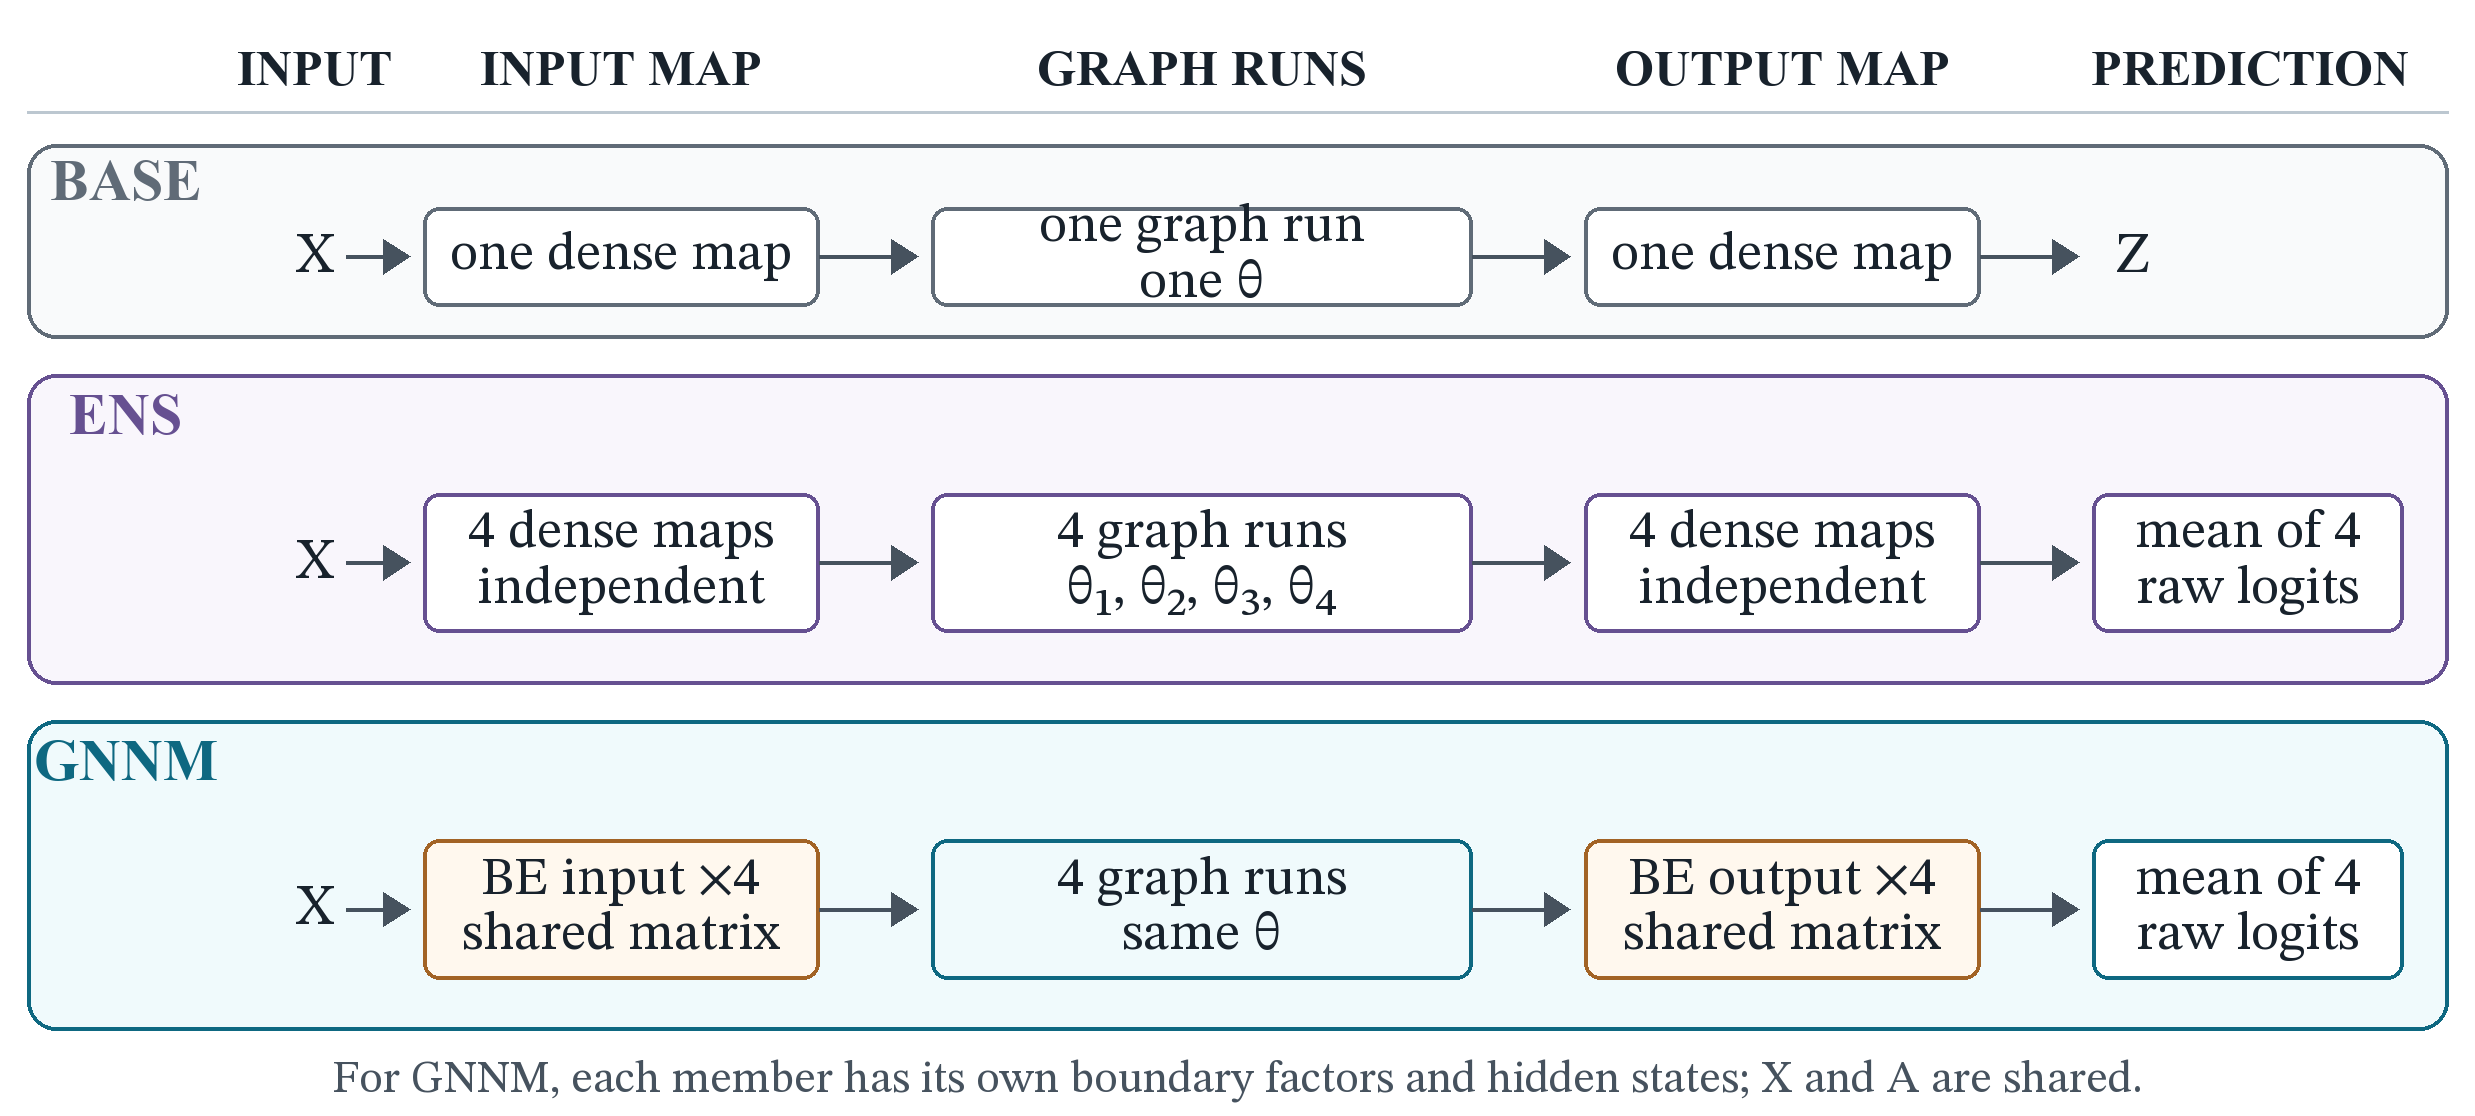
\includegraphics[width=\linewidth]{architecture_sharing_compact.png}
\caption{BASE produces one prediction. ENS stores and runs four complete models. GNNM stores one graph stack but applies it to four member-specific hidden states. The input and output matrices are each shared, with lightweight factors distinguishing the members' projectors. ENS and GNNM average the four raw output scores.}
\label{fig:sharing}
\end{figure}

Training minimizes mean member cross-entropy. All member losses update the common graph weights, while each member's factors receive their own gradients; dropout masks are drawn separately. The original benchmark averages raw logits at inference, choosing the largest score for multiclass prediction and using the averaged binary score for ROC-AUC. Its checkpoint and depth-selection procedures are specified below. The later native SAGE studies use probability averaging under their stated protocol.

The shared graph stack and projector matrices are stored once, with short private factor and bias vectors. This reduces weight storage while retaining member activations and graph computation. Appendix~\ref{app:implementation} gives exact operations, initialization and parameter counts.

\section{Five-dataset benchmark}\label{sec:original-benchmark}
\subsection{Experimental setup}
The benchmark uses the five datasets introduced by \citet{platonov2023critical} to evaluate learning on graphs where neighboring nodes need not share labels. Roman Empire and Amazon Ratings are multiclass tasks evaluated by accuracy. Minesweeper, Questions and Tolokers are binary tasks evaluated by ROC-AUC. Each dataset supplies ten official train/validation/test splits.

We use seven graph backbones: GCN, SAGE, GAT, GAT-sep, GT, GT-sep and TAG, plus a graph-free ResNet control. GT denotes the TransformerConv-based implementation specified in the appendix. For every backbone, BASE is one ordinary model, ENS is four independent ordinary models, and GNNM uses four member paths. This compares sharing within each architecture instead of combining different backbones into one ensemble.

All benchmark models use hidden width 512, learning rate $3\cdot10^{-5}$, AdamW with zero weight decay, LayerNorm, GELU and dropout 0.2. Depths 1--5 are evaluated, and validation chooses a depth separately for each method and official split. Runs have a 5,000-step cap and validation stopping. The supplement reconstructs the complete grid from 6,000 original run records and identifies all 1,200 selected records.

Each method uses its intended validation procedure. ENS trains its members independently and selects each member's checkpoint using its own validation score, then chooses depth using their averaged prediction. GNNM trains its four paths jointly and selects one model checkpoint using their averaged validation prediction. Both procedures use validation data to select predictions evaluated on the test split. The benchmark compares these complete methods as designed. To study the effect of shared graph weights by itself, we use separate matched comparisons below. Projector initialization also differs in the original benchmark, and its launch-time code and data fingerprints were not preserved. Appendix~\ref{app:protocol} gives the exact reconstruction rule and provenance limits.

\subsection{Predictive results}
\begin{figure}[t]
\centering
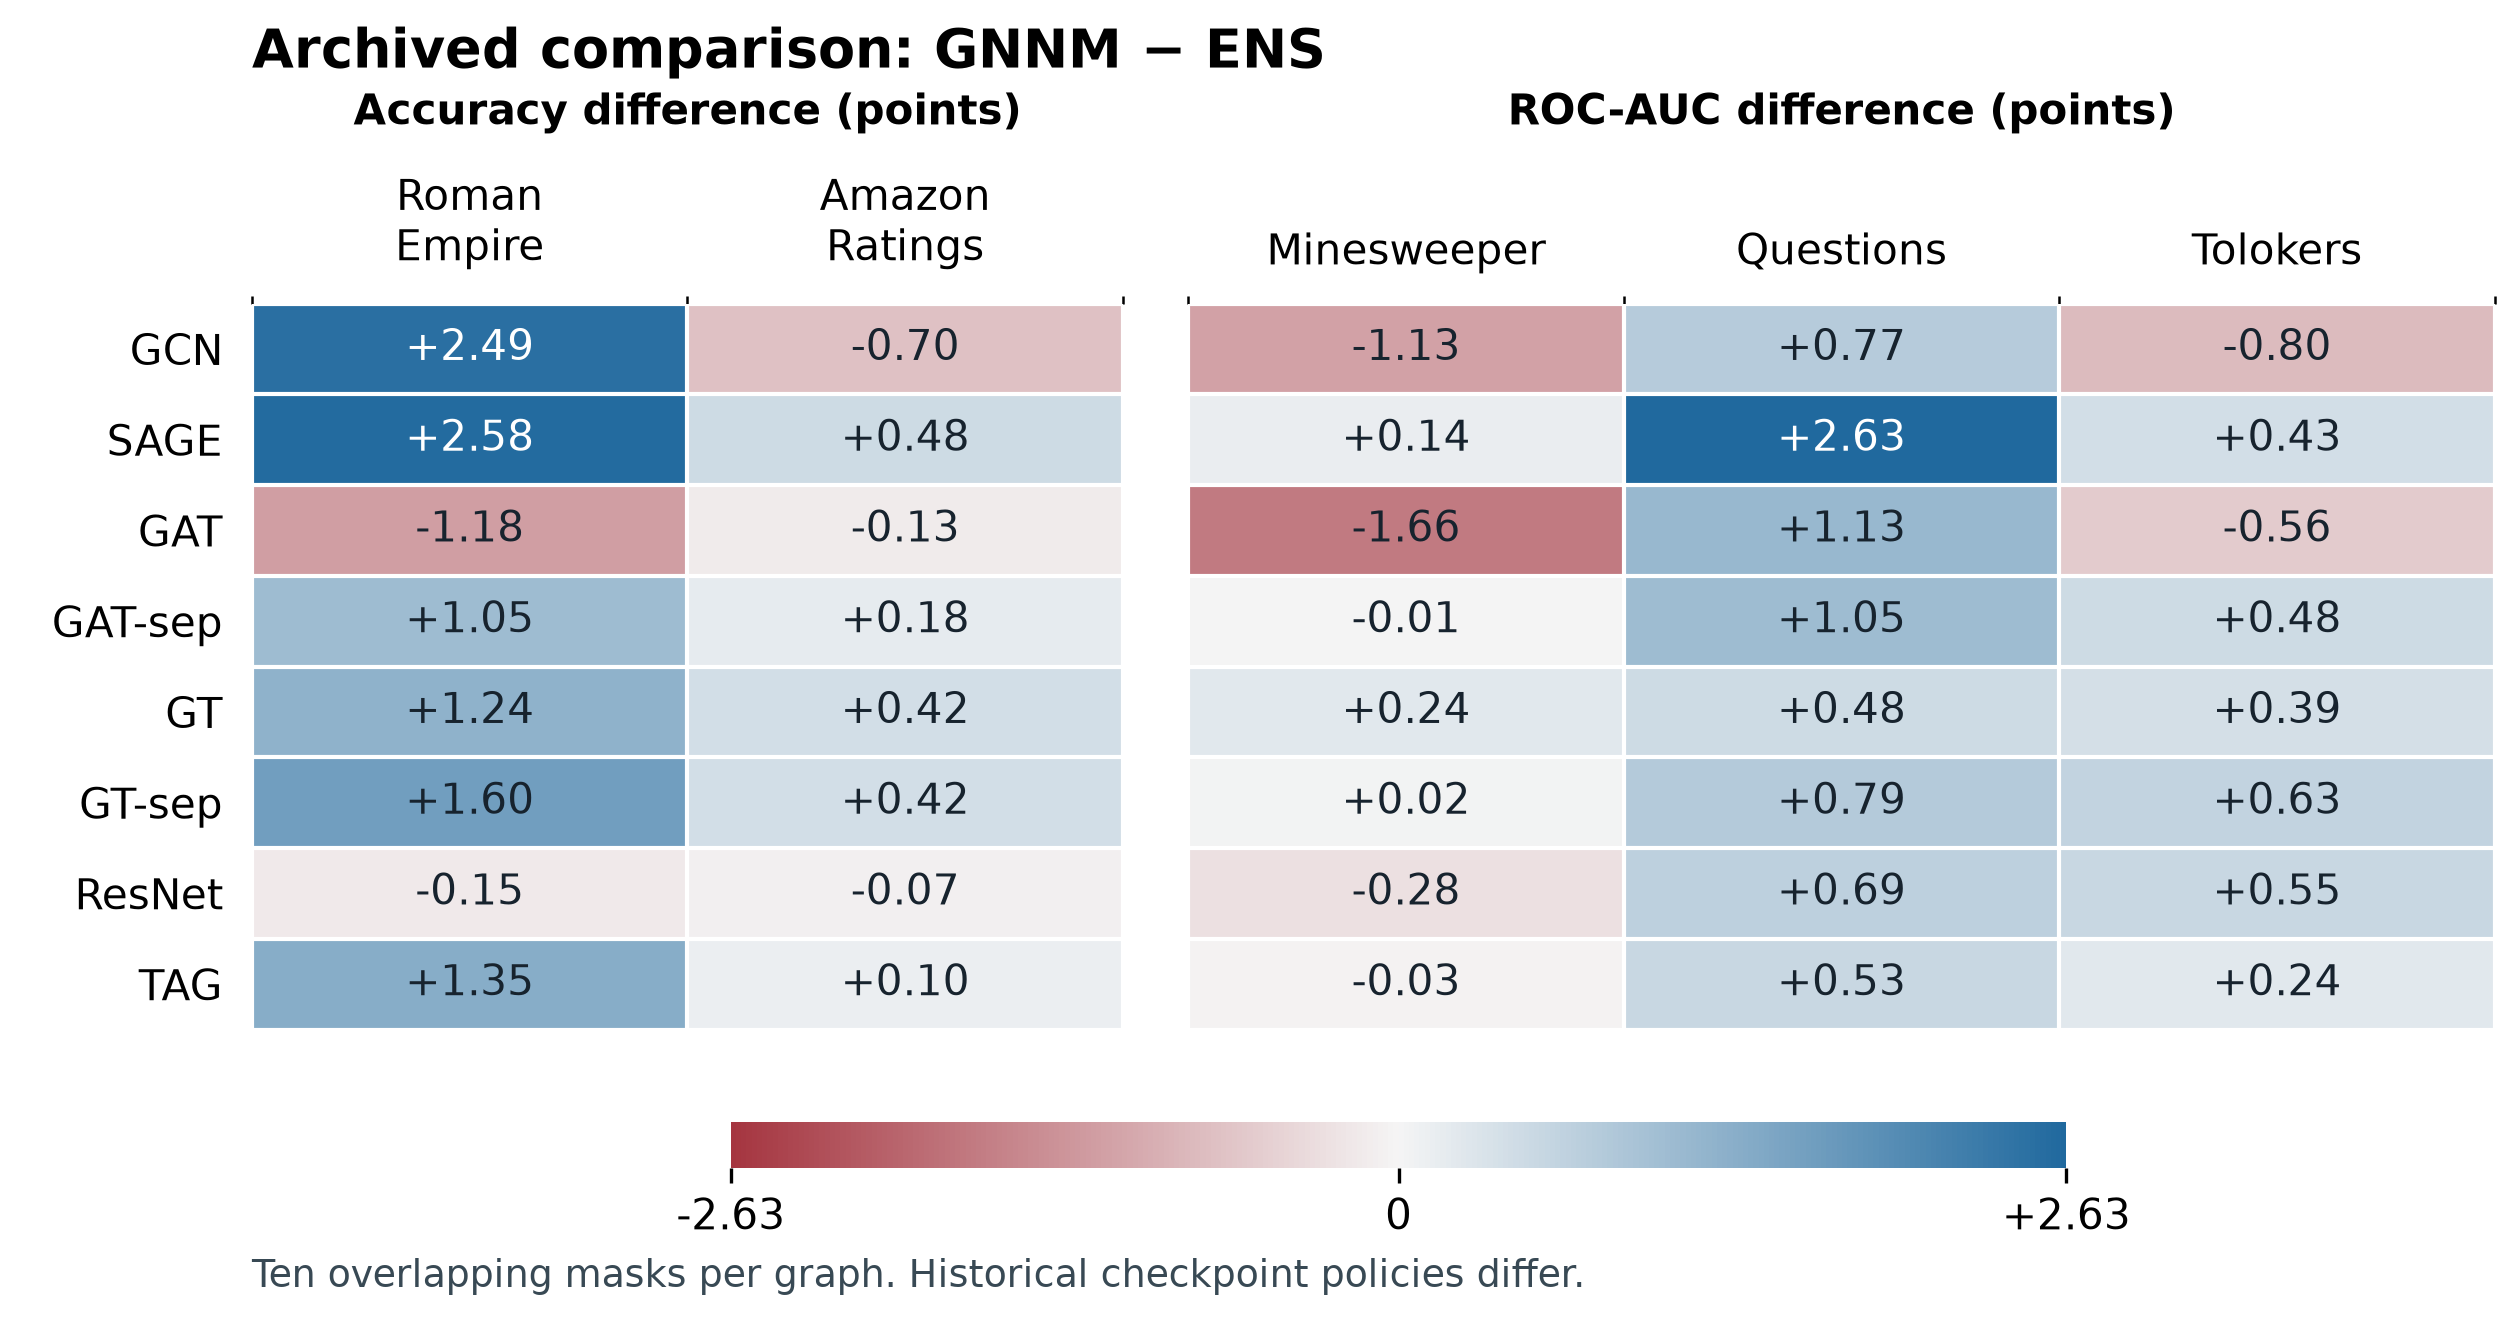
\includegraphics[width=\linewidth]{gnnm_vs_ens_heatmap.png}
\caption{GNNM minus the four-model ensemble on all five datasets and eight backbones. Each cell averages the paired differences over ten official splits, in percentage points of that dataset's metric. Blue favors GNNM and red favors ENS. The two metric families are shown separately. Each method uses its intended validation-selection rule. Appendix Table~\ref{tab:benchmark-absolute} gives all absolute scores and deviations.}
\label{fig:benchmark-main}
\end{figure}

Figure~\ref{fig:benchmark-main} shows every dataset and backbone. GNNM exceeds BASE in 33 of 40 mean comparisons and ENS in 28. Relative to ENS, it improves on six of eight backbones on Roman Empire, five on Amazon Ratings, three on Minesweeper, all eight on Questions, and six on Tolokers. These counts summarize the suite. The 40 cells share five graphs and are not 40 independent tasks.

The most consistent backbone results are SAGE, GT and GT-sep, which improve over ENS on all five datasets. For SAGE, Roman Empire rises from 87.47\% to 90.04\%, and Questions from 74.39 to 77.02 ROC-AUC points. Gains are smaller on Minesweeper and Tolokers. GAT behaves differently: it improves on Questions but loses on the other four datasets. GCN also loses on Amazon Ratings, Minesweeper and Tolokers. Sharing therefore depends on the backbone as well as the dataset.

The ResNet control ignores graph edges and improves over ENS on two datasets. Its behavior confirms that the boundary factorization can affect predictions without message passing. The graph results need additional comparisons to determine the contribution of sharing graph weights specifically. We provide those comparisons next. The appendix retains paired split differences, including small and negative effects; complete depth-selection sensitivities are in \path{code_evidence/history/profile_and_selection_details.tex.txt}.

\subsection{Storage and execution cost}
In the original resource sweep, GNNM stores roughly one quarter of ENS's parameters. Its measured training-step time is 0.3--2.5\% higher. This is expected from the implementation: four different hidden-state tables still pass through the graph. Parameter storage is the measured benefit, while compute and peak memory must be assessed separately.

\begin{table}[t]
\centering\small
\setlength{\tabcolsep}{4pt}
\caption{Original resource sweep, averaged over eight backbones and five depths. Parameter counts are millions, step times are milliseconds, and peak allocation is MiB. These configurations are not necessarily the depth selected for prediction. Both methods use four paths.}
\label{tab:resource-main}
\begin{tabular}{lrrr}
\toprule
& Parameters & Step time & Peak allocation\\
Dataset & ENS / GNNM & ENS / GNNM & ENS / GNNM\\
\midrule
Roman Empire & 16.04 / 4.02 & 204.4 / 209.6 & 2228 / 2164\\
Amazon Ratings & 16.01 / 4.01 & 300.7 / 306.5 & 3706 / 3636\\
Minesweeper & 15.40 / 3.86 & 126.8 / 128.5 & 1679 / 1543\\
Questions & 16.00 / 4.01 & 542.1 / 552.8 & 6385 / 6420\\
Tolokers & 15.41 / 3.86 & 658.7 / 660.6 & 12953 / 12818\\
\bottomrule
\end{tabular}
\end{table}

Table~\ref{tab:resource-main} separates these costs. The sweep uses 50 warmup steps and 200 synchronized optimization steps. It processes members sequentially and uses weight decay 0.01 for all methods, whereas predictive runs use zero decay. The original sweep records do not independently identify the device model. Later profiles use an identified A100 and saved timing samples. Appendix~\ref{app:cost-details} gives the protocols and full measurements. We do not claim lower latency or lower peak memory from fewer stored parameters.

\section{Analysis of the member paths}\label{sec:analysis}
The benchmark measures the complete GNNM recipe, which changes both the projectors and the sharing of graph weights. To examine the contribution of sharing itself, we start with GNNM and give each member its own copy of the graph stack. The copies initially contain the same values, so the member functions are matched before training. During training, the copies can change independently. Both versions choose a checkpoint using the same averaged validation prediction. Their difference measures what happens when the requirement to share graph weights is removed, under this training recipe.

We make this comparison on a favorable benchmark setting: five-layer SAGE, width 512, on Roman Empire masks 0--4. Every four-member method in Table~\ref{tab:component-main} uses the common checkpoint rule. The setting was chosen after the benchmark, so the study examines one observed success. It does not estimate the effect of sharing across new graphs.

\begin{table}[t]
\centering\small
\setlength{\tabcolsep}{5pt}
\caption{Roman Empire component study. Accuracy is mean $\pm$ standard deviation over five overlapping official masks. All four-member rows use a pooled checkpoint rule. The first two rows form the matched-initialization sharing comparison. The remaining component comparisons have the initialization relationships specified in Appendix~\ref{app:controls}.}
\label{tab:component-main}
\begin{tabular}{lrr}
\toprule
Method & Accuracy (\%) & Parameters ($10^6$)\\
\midrule
GNNM & $89.50\pm0.29$ & 6.738\\
Private propagation for every member & $86.56\pm0.57$ & 26.437\\
\midrule
Four ordinary models (pooled ENS) & $87.52\pm0.26$ & 26.923\\
Four independent input/output maps & $86.99\pm0.38$ & 7.221\\
Input factors only & $89.35\pm0.32$ & 6.736\\
Output factors only & $84.96\pm0.47$ & 6.733\\
Four output heads & $84.97\pm0.56$ & 6.758\\
Frozen output factors & $89.48\pm0.28$ & 6.736\\
Factors also inside graph layers & $89.66\pm0.14$ & 6.871\\
One-member GNNM & $85.47\pm0.64$ & 6.732\\
BASE & $86.21\pm0.47$ & 6.731\\
\bottomrule
\end{tabular}
\end{table}

GNNM exceeds the version with private graph stacks by 2.94 accuracy points on average, with positive differences on all five masks. It also exceeds the ordinary ensemble under the common checkpoint rule by 1.99 points. The private-stack model can reproduce any GNNM prediction by keeping its four graph stacks identical. GNNM's higher accuracy here therefore cannot come from access to a larger set of prediction functions. It concerns what this training and checkpoint-selection procedure finds under the sharing constraint. Giving members private weights changes both capacity and optimizer histories, which this comparison does not separate. Repeating the matched sharing comparison on mask 0 with three optimization seeds gives a gain of $3.33\pm0.63$ points (sample SD), positive for every seed. This remains evidence from one graph and a finite training budget.

Sharing weights is only part of GNNM: its members also enter the graph layers with different hidden states. To examine this distinction, we compare varying the input map with varying only the output map. The latter makes several predictions from one common propagated representation. The input-only variant scores close to GNNM, whereas output-only and heads-only variants score lower in this case. Freezing the output factors barely changes the mean, while adding factors inside every graph layer gives a small increase. This pattern is consistent with useful input variation in this setting. Several variants start from different functions, so these comparisons do not isolate a single component or establish that both boundary projectors are necessary or optimal.

A higher ensemble score can arise because its members become more accurate, because averaging corrects more of their errors, or both. We therefore return to the saved predictions from the matched sharing comparison. For each method, we calculate the mean accuracy of its four members and then the additional accuracy obtained by averaging their raw scores. This divides the observed ensemble difference into two quantities without changing any predictions.

For the Roman SAGE comparison, GNNM's members are 3.08 points more accurate than the untied members on average. Its gain from averaging is 0.14 points smaller. Together these changes give the 2.94-point pooled advantage. Pairwise class disagreement falls from 8.00\% to 6.07\%. Thus this favorable result comes from better members despite lower measured disagreement. More disagreement alone is not a sufficient explanation of ensemble quality.

A parallel comparison with Roman GAT checks whether this SAGE pattern also appears in an attention backbone. The mean shared-minus-private difference is only 0.04 points, with mixed signs across masks. The original GAT losses therefore do not reproduce as a large penalty from sharing in this case. Together, these results locate a favorable SAGE effect and prevent its member-accuracy explanation from being applied to every backbone. They describe the selected predictions, without establishing why training finds them. Appendix~\ref{app:gat-pair} gives the GAT masks and decision counts.

\section{Internal SAGE sharing under stronger references}\label{sec:internal-sage}
We next compare a shared bank against capable singles and complete ensembles when member factors also enter the native SAGE maps. This internal-factor version differs from the original boundary projectors: it factorizes every native dense map and retains shared native biases. Four complete route states train with mean own cross-entropy and serve the mean class probabilities. The two-block, width-128 procedure and its five arms are specified in Appendix~\ref{app:internal-sage-F}.

On selected WikiCS development, Shared4 gains 0.7205 percentage points over matched joint untied4 and 0.5372 over genuine factorized I4, with positive differences at all three seeds. Descriptive paired-seed 95\% intervals are $[0.2712,1.1698]$ and $[-0.2653,1.3398]$ points, respectively. Both ordinary and factorized single references are reported in Table~\ref{tab:internal-sage-F}. These are three optimizer repeats on the same 5,274 nodes used for checkpoint selection and subsequent calibration.

Shared4's average member is weaker than either ensemble control. Against I4, 225 additional covered readouts are offset by 141 additional pooling losses; one aggregation-only correction leaves 85 more correct decisions (Figure~\ref{fig:internal-members-coverage}). Higher calibrated NLL accompanies the raw accuracy gain, while calibrated Brier improves. The predeclared mean-NLL allowance fails against I4 (Appendix~\ref{app:internal-sage-F-gates}). This differs from Roman SAGE's stronger-member explanation and remains selected development evidence. The next study tests whether transforming the neighbor values improves this shared bank's predictions.

\section{Conditional neighbor values and packed controls}\label{sec:conditional-values}
The preceding study leaves a member-quality limitation: sharing can improve the pool while its members remain weaker than independently acquired models. E4 changes the scores upstream of pooling by transforming nonself neighbor values before the native SAGE mean. Shared affine builders use live source and receiver states to produce paired maps; private factors distinguish their member routes. Factual support, self values and the remaining native computation are retained. Conditional filtering and endpoint maps have established ancestry \citep{simonovsky2017ecc,brockschmidt2020film,bodnar2022sheaf,bourgerie2026deepnsd}; this comparison tests their placement within shared native SAGE.

The same endpoint operation equips a factorized single and four genuinely independent models. N4 has the same parameters and matrix action, but uses only the receiver state and its SiLU transform. It provides the control for source conditioning. BASE is a fresh unchanged internal-factor shared bank. Training, selection and probability averaging follow the fixed own-loss recipe; the earlier F study remains separate. Appendix~\ref{app:E-PE} gives exact operations, controls, calibration and costs.

\begin{table}[t]
\centering\small\setlength{\tabcolsep}{6pt}
\caption{Complete conditional-SAGE and packed comparison on selected WikiCS development. All entries are three-seed means; lower NLL is better. The full member, Brier, calibrated and resource results are in Appendix~\ref{app:E-PE}.}
\label{tab:E-PE-main}
\begin{tabular}{lrrr}
\toprule
Arm & Raw accuracy (\%) & Raw NLL & Parameters\\
\midrule
BASE (fresh shared4) & 80.6282 & 1.1380 & 216,674\\
E4 (endpoints) & 81.1971 & 0.7611 & 237,474\\
N4 (receiver) & 81.0517 & 0.7378 & 237,474\\
Equipped M1 & 80.2174 & 0.7653 & 225,600\\
Equipped I4 & 80.8937 & 0.6888 & 902,400\\
PE4 (width 59) & 79.7876 & 0.6956 & 215,508\\
\bottomrule\end{tabular}\end{table}

E4 reaches 81.1971\% raw pooled accuracy, versus 80.6282\% for BASE and 80.8937\% for equipped I4. Paired gains are 0.5688 points with descriptive 95\% interval $[0.1146,1.0231]$ and 0.3034 points with interval $[-0.3560,0.9628]$, respectively. All three seed differences are positive, but the I4 interval includes zero. E4's raw and calibrated NLL and Brier are worse than I4's. Its mean calibrated-NLL harm of 0.0160 passes the predeclared practical allowance; that practical screen is distinct from a noninferiority conclusion. The same development nodes informed native selection before calibration, so this is not unused confirmation.

N4 reaches 81.0517\%, accounting for about 74\% of E4's BASE gain, with slightly stronger average members. The endpoint increment is 0.1454 points, with descriptive interval $[0.0015,0.2893]$. Relative to BASE, E4's mean members improve 1.0729 points. Coverage falls by 106 readouts while pooling losses fall by 196, leaving 90 more correct pooled decisions. Its mean members remain 0.7632 points weaker than equipped I4. These counts repeat the same 5,274 development nodes across three seeds and describe separately fitted and selected procedures.

A common-rival error limits what unchanged scalar pooling can recover. If some false class strictly exceeds truth in every member's raw scores, exact softmax preserves that ordering in every member probability, and any nonnegative scalar probability average preserves it too. E4 has this predicate on 2,064 of its 2,975 pooled-error readouts. Other errors include correct member alternatives lost in pooling. The predicate does not show absent hidden information, and removing it is not necessarily a served repair. A completed probe with zero-anchored private affine heads fails its frozen private-specific and untouched-E improvement criteria and serves no repair of those original rival errors (Appendix~\ref{app:E-error-head}). This closes that fixed-feature recipe, without establishing a global head-capacity limit.

A forward-only source-association diagnostic reassigns source context while retaining actual neighbor values, receiver context, self records and support at each intervention hook. Reassigning both layers lowers E4 accuracy by 0.2844 points and I4 by 0.0822; their mean member losses are similar. The E--I4 served gap contracts from 48 to 16 readouts while its coverage gap grows from 44 to 59 and relative pooling losses worsen from $-4$ to 43. E layer 0 loses accuracy while improving NLL. This is selected-function dependence under one restricted mapping, with downstream states allowed to change. It establishes neither a learning cause nor private-builder necessity (Appendix~\ref{app:association-v5}).

For storage context, we adapt Packed-Ensembles with four untied width-59 SAGE bodies and $\gamma=1$ \citep{laurent2023packed}. Width is fixed by BASE's full parameter cap before scoring: PE4 stores 215,508 parameters, BASE 216,674, and E4 237,474. PE4 reaches 79.7876\% accuracy; E4 gains 1.4094 points, with descriptive interval $[0.9820,1.8368]$. PE4 has better raw NLL (0.6956 versus E4's 0.7611), while E4 has better raw Brier. This is one narrower packed adaptation with a coherent bank selector; the equipped full-width I4 remains the quality reference. PE calibration was not added. Equipped I4 stores 902,400 parameters. Recorded activation costs remain in the appendix; fewer stored weights supply no compute or memory advantage here.

\subsection{Native FiLM development reference}\label{sec:film}
A complete native PyG GNN-FiLM adaptation tests a richer receiver-conditioned message operator, including messagewise ReLU before averaging and the native skip \citep{brockschmidt2020film,fey2019pyg}. It uses the same WikiCS training/development population and three seeds, with equally processed factorized single, shared-four and genuinely independent-four procedures. The shared bank reaches 79.9836\% raw accuracy and I4 78.4161\%, versus E4's 81.1971\%. E4's paired gains are 1.2135 and 2.7809 points, with descriptive 95\% intervals $[0.1913,2.2357]$ and $[2.1414,3.4204]$; raw and calibrated NLL and Brier also favor E4 in this setup. Shared FiLM itself gains 1.5674 points over its I4, with stronger mean members, while raw NLL worsens and calibrated NLL improves. All nine banks, eighteen fits and forty-five temperature fits close (Appendix~\ref{app:film-v5}).

Native FiLM differs from N4 and E4 in operator, geometry and capacity: its shared bank stores 354,146 parameters versus E4's 237,474. Its tested single and independent scores are below the capable E-family references. These adaptation outcomes are exploratory encountered-development comparisons, without capacity matching, published-score reproduction, multiplicity-adjusted superiority or unused confirmation. They establish no general inferiority of conditional filtering.

\section{Complete heldout studies}\label{sec:heldout}
The WikiCS studies informed these two prospectively fixed procedures. Each closes all selected native states before separate calibration, then releases heldout labels once for complete scoring. Physics tests conditional E; Penn94 tests internal-factor sharing. They evaluate different candidates on one additional graph each. Appendix~\ref{app:complete-confirmation-v5} gives exact roles, preprocessing, selectors, all primary vectors, multiplicity rules, proper scores and costs.

\subsection{Conditional SAGE on Physics}\label{sec:physics}
On the complete Coauthor Physics graph, ten custom class-stratified mask/optimizer blocks compare E4, unchanged BASE, receiver-only N4, equipped M1/I4 and a source-derived mean-SAGE single \citep{shchur2018pitfalls}. Each block separates 100 training, 150 selection, 150 calibration and 34,093 heldout nodes. All sixty banks, ninety selected body states and sixty fixed temperature endpoints close with finite raw and calibrated outcomes. The frozen primary rule requires both E--BASE and E--I4 to pass Holm-adjusted one-sided paired $t$ tests at 0.05 and each observed mean gain to reach 0.2 points.

E4 reaches 91.3264\% raw accuracy versus BASE's 90.5403\%, a gain of 0.7861 points with paired 95\% interval $[0.5548,1.0173]$, ten positive differences and Holm $p=3.0308\cdot10^{-5}$. Equipped I4 reaches 92.7891\%: E4 loses 1.4628 points, with interval $[-1.8744,-1.0511]$ and ten negative differences. The joint primary criterion fails. Equipped M1 (92.2233\%) and the source-derived mean-SAGE single (93.0590\%) are also stronger accuracy references; the latter has its own architecture and selection budget and is not an exact published-split reproduction.

E--N gains only 0.0282 points with interval $[-0.0972,0.1535]$ and six positive/four negative differences. Its conditional attribution gate remains closed. E4 has worse raw and calibrated NLL and Brier than equipped I4; calibrated-NLL harm is 0.061336 on average, exceeding the 0.02 mean allowance and the 0.05 allowance in seven blocks. This practical protection fails independently of the raw-accuracy result. Thus Physics confirms a benefit over this unchanged shared baseline, while failing the declared independent-ensemble and endpoint-attribution claims. Selected WikiCS sensitivity cannot rescue this outcome.

\subsection{Internal factors on Penn94}\label{sec:penn}
Penn94 retains official split-0 test membership: 9,705 heldout nodes. Ten paired optimizer blocks compare internal shared4 with original boundary GNNM, genuine internal-factor I4, ordinary M1 and factorized M1; matched boundary sharing and LINKX provide separate placement and task context. Training uses 19,407 nodes; the official validation set is prospectively divided into 4,852 selection and 4,851 calibration nodes. Target information is removed from input features. All seventy banks, one hundred body attempts, ninety bank/fusion calibration endpoints and ninety confirmation rows close with zero native or calibration failures. The primary rule requires all four contrasts to have an observed gain of at least 0.2 points and Holm-adjusted one-sided paired $t$ values at most 0.05.

Internal shared4 reaches 78.1535\% raw accuracy versus I4's 75.2993\%, gaining 2.8542 points with paired 95\% interval $[2.5464,3.1620]$, ten positive differences and Holm $p=8.9307\cdot10^{-9}$. Its mean members improve 2.1602 points. Gains over ordinary and factorized singles are 3.5930 and 3.5415 points. Original boundary GNNM reaches 79.1334\%: internal sharing loses 0.9799 points, with interval $[-1.4908,-0.4690]$, nine negative differences and one tie. The all-four primary criterion therefore fails. LINKX reaches 84.6852\%, above every SAGE procedure, and remains descriptive task context outside the tested families.

Original GNNM uses one-logit binary cross-entropy, raw-logit pooling, its original initialization/global random stream and checkpoint cadence, with a 5,000-update ceiling. Internal sharing uses two-logit cross-entropy, probability pooling and a 1,000-update ceiling. Their contrast compares whole recipes. Under common acquisition, internal probability pooling gains 0.2916 points over matched boundary probability pooling, but the secondary confirmatory gate is closed. On the same selected internal and matched boundary states, probability pooling loses 0.1484 and 0.1216 points to logit pooling. These descriptive alternatives do not validate a newly selected pipeline or replace the frozen heldout criterion.

Internal sharing's raw NLL is 0.453237 worse than I4 despite better Brier. One positive temperature fitted for each bank/fusion on the separate calibration role reduces its NLL difference to $-0.035860$. All four practical calibrated-NLL protections pass, without establishing statistical noninferiority or removing raw overconfidence. Penn shows a strong conditional benefit over the declared singles and independent internal-factor ensemble, while retaining stronger original GNNM and LINKX and a failed complete primary criterion. It is not a replication of conditional E.


\section{Scope across sharing placements and budgets}\label{sec:additional}
An ordinary ensemble can also store fewer weights by making each member narrower. A useful storage comparison must therefore give this smaller ensemble a similar parameter budget. On Roman SAGE, we choose its width by parameter count before scoring: four width-256 models contain 6.908 million parameters, close to width-512 GNNM's 6.738 million. GNNM scores 89.50\% versus 88.14\%, but inference takes 109.7 ms versus 39.9 ms. In this setting, sharing allows wider member states and higher accuracy within a similar weight budget, at the cost of longer computation. A wider single model chosen by training-step time also scores lower, although its complete training finishes sooner (Appendices~\ref{app:param-matched} and~\ref{app:strong-base}).

Additional two-block SAGE studies compare full sharing with variants having one private graph block, either first or last, under validation-selected optimizer settings. Full sharing improves only WikiCS in the four-graph primary grid. Selected partial sharing nearly ties ENS on raw Cora, improves WikiCS, and loses on Actor, filtered Chameleon, CiteSeer and PubMed; normalizing Cora changes its outcome. Appendix~\ref{app:sharing-scope-summary} retains the contrasts and failures; complete selected/default grid tables are in \path{code_evidence/history/secondary_grid_and_optimizer.tex.txt}.

At similar stored-weight budgets, selected private-last models improve WikiCS and normalized Cora with higher measured inference latency (Tables~\ref{tab:wikics-matched-budget} and~\ref{tab:cora-matched-budget}). These graph, placement and preprocessing choices followed earlier outcomes. Appendix~\ref{app:sharing-scope-summary} summarizes the numerical contrasts and limits; Appendix~\ref{app:validation-tuning} gives the full optimizer protocol. No rule for choosing sharing on a new graph has been validated independently.

\section{Related work}
Deep ensembles train and average independent predictors \citep{lakshminarayanan2017simple}. TreeNets share early computation before branching \citep{lee2015heads}. GNNM instead creates distinct member states before graph propagation and shares the weights applied to those states. BatchEnsemble provides the multiplicative factorization \citep{wen2020batchensemble}, and TabM studies related models for tabular data \citep{gorishniy2025tabm}. Kim's master's thesis applies BatchEnsemble inside GNN layers \citep{kim2023efficient}. Its bibliographic record is supplied, and our added-factor comparison is not an exact reproduction of that implementation.

Conditional messages and learned endpoint maps also precede E. ECC generates filters from edge information \citep{simonovsky2017ecc}; GNN-FiLM modulates source messages using receiver features \citep{brockschmidt2020film}; NSD and Deep NSD learn paired endpoint maps \citep{bodnar2022sheaf,bourgerie2026deepnsd}. Our native FiLM adaptation uses its own full message operator and supplies a fixed-recipe comparison, with different capacity and geometry. Bayesian Sheaf Neural Networks already combine one learned network with predictive ensembling over sampled sheaf geometry \citep{gillespie2025bsnnv2}. Version 2, dated 12 September 2025, describes its architecture in Section 3.4; official proceedings or journal publication remains unverified. E instead uses persistent point-estimated route factors and live endpoint-conditioned native values, without a sheaf-posterior objective. This difference supplies no broad shared-network/private-geometry novelty claim. The primary method of GENN \citep{duan2024graph} remains unread and unresolved in the present evidence, so its overlap cannot be excluded.

Other approaches target different costs. GEENI approximates constituent GNNs to reduce ensemble latency \citep{nagarajan2022geeni}, and ensembles can be distilled into one predictor \citep{zhang2024e2gnn}. Graph mixtures learn how to choose or weight experts \citep{wang2023graph,deng2025mixture}, whereas GNNM uniformly averages member scores. MIMO trains multiple predictions within one forward pass \citep{havasi2021training}, while Packed-Ensembles use grouped operations to run structured ensembles together \citep{laurent2023packed}. The native SAGE comparison includes one parameter-budget Packed-Ensembles adaptation. MIMO and the other untested efficient methods remain relevant alternatives; the experiments do not establish a general efficiency ranking. The tested alternatives include the local MC Dropout comparison in Appendix~\ref{app:mc-dropout}, with complete context in \path{code_evidence/history/roman_sensitivities.tex.txt}.

\section{Limitations and conclusion}
The original five-dataset benchmark favors GNNM most consistently for SAGE and the two graph-transformer variants, with losses in other backbones. Matched Roman SAGE gains through stronger members despite lower disagreement. Internal sharing on WikiCS gains through broader coverage despite weaker members and a failed mean calibrated-NLL allowance. On Penn94 it instead improves member accuracy over its independent counterpart, but original GNNM and LINKX remain more accurate. Conditional E improves its WikiCS BASE and the tested native FiLM procedures on encountered development. Its small advantage over equipped WikiCS I4 is uncertain and has worse proper scores. On heldout Physics it loses to equipped I4 and the source-derived single-model reference, and fails the I4 calibrated-NLL protection. The complete Physics and Penn primary criteria both fail; favorable contrasts and WikiCS diagnostics do not rescue them.

These are complete procedures built from established components, with evidence limited by graph, recipe and selection history. Historical launch-time source/data fingerprints are incomplete. WikiCS development nodes informed native selection before calibration and diagnostics. Physics and Penn separate training, selection, calibration and heldout scoring, but each supplies one additional graph with ten conditional optimizer or mask/optimizer blocks, not ten independent tasks. Sharing can strengthen members or alter retained alternatives; no universal weaker-member or gradient-cancellation account follows. The association diagnostic measures selected-function dependence under one restricted mapping, and the exact affine-head recipe fails. Private-builder necessity and a general learning mechanism remain unestablished. Sharing placements, budgets and proper scores include failures. Multiple graph trajectories and conditional-builder activations remain paid computation; fewer stored weights imply neither lower latency nor lower peak memory.

\section*{Reproducibility statement}
The appendix specifies model definitions, optimization and checkpoint-selection rules, complete benchmark scores, development outcomes and full Physics/Penn confirmation outcomes, including failed gates, paired vectors, uncertainty, proper scores and cost scopes. Named files in \path{code_evidence/} retain the relocated historical operations, grids and accounting, the complete V3 archive and inherited V4 metadata. \path{evidence/} contains the closed E/PE, head, association, native FiLM and heldout scalar/custody records. \path{IMMUTABLE_DEPENDENCIES.json} binds their exact source files and receipts; the source bundle contains no new dataset, checkpoint or logit tensors. Original run results, validation traces, selection locks and selected predictions remain preserved in the accompanying research evidence. Historical launch-time model-source, environment and exact data fingerprints are incomplete, preventing exact replay of the original benchmark training runs.

\section*{AI use statement}
OpenAI Codex was used during earlier research and manuscript preparation for literature search, editing, draft critique, the architecture figure, experimental implementation and data preparation, and artifact audits. The authors checked numerical claims against preserved run records or completed experiments and are responsible for the final text, code, analyses and citations.

\bibliographystyle{iclr2027_conference}
\bibliography{references,references_additions}
\clearpage
\appendix
\renewcommand{\thesection}{A\arabic{section}}
\renewcommand{\theHsection}{appendix.\arabic{section}}
\renewcommand{\thefootnote}{\arabic{footnote}}
% Condensed historical paper appendix; complete earlier bytes remain in code_evidence/v3_archive.
\section*{Appendix guide}
The paper appendix retains model and selection rules, absolute benchmark results, fixed-mask vectors, uncertainty, resource scopes and adverse findings. Longer historical detail and secondary grids are supplied as named plain-text files in \path{code_evidence/}; the complete earlier source and its records are preserved in \path{code_evidence/v3_archive/}, while the compact upload omits full trained checkpoints.

\section{Method, implementation, and exact scope}\label{app:implementation}
The input and output BatchEnsemble projectors use shared bias-free matrices
with Xavier-uniform initialization. An input factor $r_m$ starts with
independent equiprobable signs; its output scale starts at one and bias at
zero. All output-projector factors start at identity scale and zero bias.
Input-projector output receives dropout $0.2$ and GELU. LayerNorm precedes
the output projector. Four member losses are averaged during training;
raw member logits are averaged for checkpoint selection and inference.
Multiclass tasks use cross-entropy and binary tasks use binary
cross-entropy with logits. Each member propagates a distinct hidden state.

The supplied code uses residual native convolutions, with concatenated self/convolution values for SAGE and GAT-sep; ResNet has no graph operation \citep{kipf2017semi,hamilton2017inductive,velickovic2018graph,du2017topology,brody2022how,fey2019pyg}. TAG uses three hops. GT/GT-sep use TransformerConv with its internal root skip and separate feed-forward residuals; their output maps use convolution values alone or concatenated self/convolution values, respectively \citep{shi2021masked}. Width-512 attention uses eight heads and coefficient dropout 0.2. Historical configured convolutions do not duplicate loader self-loops; the newer SAGE grid adds none. Exact operations are in \path{code_evidence/history/native_operations.tex.txt}; they describe supplied code, without recovered launch-time source hashes.

BASE uses ordinary dense projectors with PyTorch default initialization
and bias. An $M=1$ BatchEnsemble model therefore is not an exactly
initialization-matched BASE. A four-member explicit ensemble can represent
every deterministic GNNM inference function by copying the common graph
weights into four ordinary models and replacing each boundary projector
with its member's effective dense map. This inclusion concerns function
representation and says nothing about what training finds.

\section{Equal-grid node comparisons and matched sensitivities}\label{app:validation-tuning}
Cora, WikiCS split 0, Actor split 0 and official filtered Chameleon split 0 use source features/masks and coalesced bidirectional edges without self-loops; symmetrizing Chameleon changes its directed-edge convention. Each arm has two residual SAGE blocks, width 128, LayerNorm and dropout 0.2. BASE/ENS use ordinary starts; TIED, private-first/last and UNTIED match canonical projector values and post-construction RNG states. UNTIED copies every graph block, while the partial variants privatize only their named block.

Each arm receives six candidates: learning rates 0.0003/0.001/0.003 crossed with AdamW decay 0/0.01, three seeds and 1,000 full epochs. A nonfinite seed invalidates its candidate. Checkpoints maximize pooled validation accuracy, then minimize cross-entropy, then choose the earliest epoch; candidates rank their three-seed means, then lower rate/decay. Validation chooses between two complete partial-arm searches, giving that family twice ENS's search. The 432-cell grid was locked before all 141 allowed selected/default score records; default is rate 0.001 and zero decay. Reused public splits, cap-adjacent checkpoints and unmatched stacks across the two A100 hosts limit generalization and convergence claims; arms share a runtime within each graph.

The complete selected/default primary, citation-extension and preprocessing tables are in \path{code_evidence/history/secondary_grid_and_optimizer.tex.txt}. Their numerical contrasts and adverse conclusions remain summarized in Appendix~\ref{app:sharing-scope-summary}.

\subsection{Paired decisions and additional graphs}\label{app:paired-decisions}
Paired counts describe both-correct, candidate-only, reference-only and neither-correct readouts; reused nodes/seeds do not supply independent trials. The descriptive intervals below condition on their selected setting and omit candidate-selection uncertainty.

\begin{table}[t]
\centering\small
\caption{Illustrative paired optimizer-seed intervals for selected partial sharing minus selected ENS. Each row uses three paired seeds on one fixed graph split. The interval is the mean plus or minus $t_{0.975,2}\,\mathrm{SD}/\sqrt{3}$, with $t_{0.975,2}=4.30265$. It assumes independent approximately normal optimizer-seed differences and conditions on the frozen setting. Candidate selection used these seeds' validation outcomes, which this calculation does not account for. These are not intervals over graph tasks or nodes, or simultaneous intervals.}
\label{tab:conditional-seed-intervals}
\setlength{\tabcolsep}{4pt}
\begin{tabular}{lrrl}
\toprule
Setting & Mean $\Delta$, pp & SD, pp & Conditional 95\% interval, pp\\
\midrule
Primary Cora raw & $+0.067$ & 1.041 & $[-2.519,+2.652]$\\
Primary WikiCS & $+0.741$ & 0.240 & $[+0.146,+1.336]$\\
Primary Actor & $-0.439$ & 1.259 & $[-3.567,+2.689]$\\
Filtered Chameleon & $-3.093$ & 5.809 & $[-17.523,+11.338]$\\
CiteSeer & $-1.833$ & 1.168 & $[-4.734,+1.067]$\\
PubMed & $-0.867$ & 0.643 & $[-2.464,+0.730]$\\
Cora raw repeat & $-0.133$ & 1.002 & $[-2.622,+2.355]$\\
Cora normalized & $+2.433$ & 1.801 & $[-2.040,+6.907]$\\
\bottomrule
\end{tabular}
\end{table}

\subsection{Citation extensions and preprocessing}\label{app:planetoid-confirmation}\label{app:cora-preprocessing}
The same grid adds 216 CiteSeer/PubMed runs on row-normalized public splits; selected partial sharing loses to ENS at every seed on both graphs. A separate 216-run Cora sensitivity reuses its public split: raw features leave selected partial sharing near ENS, whereas row normalization favors private-last by 2.433 points. The raw TIED result is 67.700\%, versus 66.900\% in the separate factor-placement repeat despite matched effective data and model bodies; initial-logit hashes differ and the cause remains unresolved. All common-default TIED scores/selected epochs reproduce exactly. Full original tables, both outcomes and preprocessing records remain in the named secondary-grid file.

\section{Additional optimization checks}\label{app:optimizer-history}
SYNC maintains equal graph weights but gives each member private AdamW moments, averaging proposed weights after each update; NORM-SYNC additionally matches update length to a mean-gradient reference on its own trajectory \citep{yang2023adatask}. The locked 96-cell grid and 12-cell norm study supply no consistent accuracy improvement. Exact search and operation detail are in \path{code_evidence/history/secondary_grid_and_optimizer.tex.txt}; the fixed-recipe outcomes remain below.

\begin{table}[t]
\centering
\caption{One fixed optimizer recipe on each graph. Test accuracy is mean $\pm$ sample SD over three optimization seeds on one split. All arms use learning rate 0.001, zero decay, and 1,000 epochs. TIED, SYNC and NORM-SYNC have the same inference function class. UNTIED has separate graph stacks. Each graph's comparison uses one runtime.}
\label{tab:optimizer-default}
\small
\setlength{\tabcolsep}{4pt}
\begin{tabular}{lrrrr}
\toprule
Graph & TIED & SYNC & NORM-SYNC & UNTIED\\
\midrule
Cora & $67.733 \pm 2.558$ & $66.367 \pm 2.290$ & $67.167 \pm 1.955$ & $72.567 \pm 0.808$\\
WikiCS & $79.043 \pm 0.532$ & $78.901 \pm 0.420$ & $79.095 \pm 0.326$ & $79.055 \pm 0.288$\\
Actor & $37.303 \pm 0.822$ & $37.215 \pm 1.133$ & $37.193 \pm 1.238$ & $37.390 \pm 1.395$\\
Filtered Chameleon & $38.832 \pm 2.543$ & $39.003 \pm 2.083$ & $37.629 \pm 2.728$ & $41.409 \pm 3.432$\\
\bottomrule
\end{tabular}
\end{table}

\section{Roman component and backbone checks}\label{app:depth-grid}
A post hoc Roman SAGE depth grid changes the tying contrast's sign between shallow and deep models; overlapping masks and longer budgets check this setting, without supplying an unseen-graph depth rule. Full sensitivities and excluded numerical attempts are in \path{code_evidence/history/roman_sensitivities.tex.txt}.

\subsection{Width-512 component control}\label{app:controls}
A distinct post hoc SAGE study uses Roman masks 0--4, depth five,
width 512, learning rate $3\cdot10^{-5}$, up to 5,000 steps and one
pooled-validation checkpoint per four-member arm. The tied and untied
stacks, frozen output factors, and added in-layer factors start from
matched constructor values; the untied arm copies the graph stack.
Validation is checked at step 1 and every ten steps, with 300-step
patience. Other component variants do not all match the initial function.
Consequently, Table~\ref{tab:component-main} describes components under one favorable
setting; it is not a one-factor causal decomposition. Population
standard deviations across overlapping masks are descriptive.

\subsection{Fixed-mask optimization repeat}\label{app:fixed-mask-v4}
The width-512, depth-five Roman SAGE pair is repeated on official mask 0
with seeds 0--2. Tied test accuracies are 89.234, 89.552 and 89.287\%,
and untied accuracies are 85.634, 85.775 and 86.675\%. The paired gain
is $3.330\pm0.628$ points, using sample SD across seeds. The untied
seed-2 checkpoint selects step 4,840 of 5,000, so this does not establish
convergence. Initial parameter values and random-generator states match.

All six final checkpoints pass replay; the source supplement retains the fixed initial-logit tolerance, failed excluded attempts, traces and selected decisions.

\subsection{Roman optimizer and width controls}\label{app:roman-optimizer}\label{app:roman-narrow}
A 24-cell depth-two/depth-five SYNC comparison retains the shallow negative and deep positive tying contrast. A narrower, approximately parameter-matched UNTIED model changes the shallow mean's sign; width also changes initialization and capacity, so this is a budget sensitivity.

\subsection{Matched GAT diagnosis}\label{app:gat-pair}
The original benchmark GAT model loses to ENS on four of five graphs. A post hoc
Roman GAT pair copies the entire attention, feed-forward and internal
normalization stack at initialization, then ties or unties it for
training on masks 0--4. Depths are 5, 5, 4, 4 and 4, width 512; each
mask has one optimizer seed and a pooled validation checkpoint.
Untying raises correct-member coverage and pooling gain on every mask,
while reducing mean member accuracy on every mask. The pooled effect
is mixed and nearly zero on average. This cannot attribute the original benchmark
ENS gap to attention or to any one cause. Selected-logit and official
node-label audits are in the supplement.

\begin{table}[h]
\centering
\caption{Post hoc Roman Empire GAT pair. Pooled columns are selected test accuracy in percent. The four differences are untied minus tied in percentage points. Member is mean individual-member accuracy, gain is pooled minus member accuracy, and oracle is the fraction of test nodes for which at least one member predicts the correct class. All statistics use the same official test nodes within each mask.}
\label{tab:gat-pair}
\setlength{\tabcolsep}{4pt}
\small
\begin{tabular}{lrrrrrr}
\toprule
Mask & Tied & Untied & $\Delta$ pooled & $\Delta$ member & $\Delta$ gain & $\Delta$ oracle\\
\midrule
0 & 82.757 & 82.351 & $-0.406$ & $-1.077$ & $+0.671$ & $+0.706$\\
1 & 82.298 & 82.527 & $+0.229$ & $-0.856$ & $+1.085$ & $+1.412$\\
2 & 81.874 & 81.592 & $-0.282$ & $-1.050$ & $+0.768$ & $+0.176$\\
3 & 82.404 & 82.439 & $+0.035$ & $-0.357$ & $+0.393$ & $+1.377$\\
4 & 82.404 & 82.633 & $+0.229$ & $-0.154$ & $+0.384$ & $+0.176$\\
\midrule
Mean & 82.347 & 82.309 & $-0.039$ & $-0.699$ & $+0.660$ & $+0.770$\\
\bottomrule
\end{tabular}
\end{table}

\subsection{Other matched comparators}\label{app:param-matched}
A parameter-count-matched explicit ENS chooses width 256 from five
candidates by trainable-parameter count before scoring; a wider BASE
chooses width 1152 by measured step time. Both keep the other Roman
SAGE settings fixed. The width choices change representation and
initialization. A fixed MC Dropout comparison likewise changes the
inference sampling rule. They are contextual resource and recipe
sensitivities, not exact causal alternatives to propagation tying.
\label{app:mc-dropout}\label{app:strong-base}

Four fixed MC Dropout draws (probability 0.2) from each selected Roman BASE checkpoint give 85.362\% with logit pooling and 85.295\% with probability pooling, versus deterministic BASE's 86.209\%; both lose on every mask \citep{gal2016dropout}. Probability pooling followed the logit analysis. This untuned setting supplies no general comparison with optimized MC Dropout; all draws, seeds and mask values remain in the Roman sensitivity file.

\section{OGB node classification and link prediction}\label{app:ogb-pilot}
The OGB tasks use the official data and splits \citep{hu2020open}.
\texttt{ogbn-arxiv} uses one official temporal split, citation edges
made bidirectional, two residual SAGE blocks of width 128, dropout
$0.2$, AdamW learning rate $0.001$ and zero decay. BASE has 187,048
weights; pooled ENS 748,192; GNNM 189,248. All arms use the same
pooled validation checkpoint rule. The 100-, 300-, and 1,000-epoch
budgets each restart from initialization and run all epochs; longer
budgets were specified after shorter-budget results. Three seeds
vary optimization on one split. At 1,000 epochs, selected checkpoints
remain late, so the order is finite-budget rather than converged.
\label{app:ogb-1000}

\begin{table}[t]
\centering
\caption{Fixed \texttt{ogbn-arxiv} SAGE configuration on one official temporal split. Test accuracy is in percent. The mean $\pm$ sample standard deviation describes three optimization seeds on the same graph. Each longer budget was specified after earlier results were known. All nine runs at each budget use pooled-validation checkpoint selection.}
\label{tab:ogb-pilot}
\setlength{\tabcolsep}{5pt}
\begin{tabular}{llrrrrr}
\toprule
Budget & Variant & Seed 0 & Seed 1 & Seed 2 & Mean $\pm$ SD & Params, $10^6$\\
\midrule
100 & BASE & 67.58 & 67.70 & 68.07 & $67.78\pm0.25$ & 0.187\\
100 & Pooled ENS & 68.12 & 68.08 & 68.32 & $68.17\pm0.13$ & 0.748\\
100 & GNNM & 64.92 & 64.05 & 64.16 & $64.37\pm0.47$ & 0.189\\
\midrule
300 & BASE & 70.84 & 70.27 & 70.81 & $70.64\pm0.32$ & 0.187\\
300 & Pooled ENS & 71.28 & 71.01 & 71.00 & $71.10\pm0.16$ & 0.748\\
300 & GNNM & 69.42 & 68.79 & 68.87 & $69.03\pm0.34$ & 0.189\\
\midrule
1,000 & BASE & 71.68 & 71.29 & 71.53 & $71.50\pm0.20$ & 0.187\\
1,000 & Pooled ENS & 72.08 & 72.25 & 72.09 & $72.14\pm0.10$ & 0.748\\
1,000 & GNNM & 71.03 & 70.65 & 70.79 & $70.82\pm0.19$ & 0.189\\
\bottomrule
\end{tabular}
\end{table}

\subsection{Frozen \texttt{ogbl-collab} extension}\label{app:collab}
The official temporal edge split uses training collaborations through
2017 to build one bidirectional propagation graph. Validation edges
from 2018 and test edges from 2019 are never added. Node features'
own temporal construction was not independently established. Four
boundary-factor paths use two residual width-128 SAGE blocks, a
128-coordinate node output and one shared three-layer decoder on the
elementwise product of endpoint vectors. UNTIED copies the initialized
graph stack. ENS has four ordinary encoder--decoder models; BASE one.

A fixed 400-step recipe uses 65,536 sampled observed training edges
and the same number of pairs absent from the training graph per step.
These candidate negatives may include future true collaborations.
All arms of a seed see the same batches. Every 20 steps a whole-model
checkpoint is ranked by official validation Hits@50, validation BCE,
then earliest step. There is no task-specific hyperparameter search.
The official test comparison is one recipe on one temporal split.
Untuned graph-only Common Neighbors and Adamic--Adar are included on
the same training graph and candidate pools. They score 41.700\% and
52.401\% Hits@50, respectively. Adamic--Adar exceeds all learned means. This study does not measure
recommendation quality.

\begin{table}[h]
\centering
\caption{Official \texttt{ogbl-collab} test Hits@50 in percent after one fixed 400-step recipe. The standard deviation is across three optimizer seeds on one temporal split. Selected steps and parameter counts are shown to expose budget and capacity differences.}
\label{tab:collab-hits}
\setlength{\tabcolsep}{4pt}
\small
\begin{tabular}{lrrrrrl}
\toprule
Variant & Seed 0 & Seed 1 & Seed 2 & Mean $\pm$ SD & Params, $10^6$ & Selected steps\\
\midrule
Tied & 48.540 & 46.662 & 46.910 & $47.371\pm1.020$ & 0.234 & 360, 360, 360\\
Untied & 47.113 & 46.196 & 47.307 & $46.872\pm0.594$ & 0.730 & 380, 360, 400\\
ENS & 43.882 & 45.688 & 44.216 & $44.596\pm0.961$ & 0.926 & 400, 400, 400\\
BASE & 37.948 & 37.331 & 40.368 & $38.549\pm1.605$ & 0.232 & 400, 360, 380\\
\midrule
Tied $-$ untied & $+1.427$ & $+0.466$ & $-0.397$ & $+0.499$ & & \\
\bottomrule
\end{tabular}
\end{table}

\section{Resource measurement}\label{app:tuning-resources}
The 24 primary selected seed-0 checkpoints were profiled on one otherwise idle A100 using three rotated blocks, each with 20 warmups and 100 synchronized full-graph inference calls: 7,200 retained calls include member forwards and raw-logit pooling, excluding loading/host transfers. Allocated peaks follow warmup; MB is decimal. Quartiles describe one checkpoint/device, and allocation excludes reserved/external memory. Full profiles are in \path{code_evidence/history/profile_and_selection_details.tex.txt}.

\section{Original benchmark provenance}\label{app:protocol}
The historical five-graph suite uses one seed on each of ten official
masks for eight backbones and three methods. For each graph and method,
we selected the unique saved result folder containing eight backbones,
five depths, ten masks, fixed width 512 and learning rate
$3\cdot10^{-5}$: 400 rows per method. This completeness rule does not
inspect test scores. The saved records do not document whether those
folders were fixed before any test inspection. For each method,
backbone and mask, the highest-validation depth supplies its test
score; validation ties within $10^{-12}$ choose the smaller depth.
The table reports mean and population standard deviation of the ten
selected scores. BASE and GNNM use the split index as the seed. ENS uses
$1000\cdot\mathrm{split}+\{0,1,2,3\}$. The runs have a 5,000-step cap
and validation stopping after approximately 300 steps without a new best.
Masks reuse nodes and are not independent graphs.

The original ENS procedure selected each independent member checkpoint
separately; GNNM selected one joint checkpoint by pooled validation.
These are the intended selection rules for the two complete methods.
BASE and ENS also use different projector initializations from GNNM.
Launch-time model-source hashes,
full software environment, and exact historical data bytes were not
preserved. In the current checkout, the Amazon Ratings file was an
HTML error; it was replaced by the official public NPZ for future
runs, with both hashes recorded. That repair does not prove the exact
historical bytes. The main benchmark is a reconstruction of the two
complete methods as run, rather than an isolated sharing intervention.
New controls use
their own stated rules. The current generic training runner's split-0
width/depth/rate search does not reproduce the original benchmark.

\subsection{Depth-selection sensitivity}\label{app:depth-sensitivity}
Retrospective rules selecting one depth from mean validation or mask-0 validation can transfer labels across overlapping masks. They are diagnostic, rather than replacement estimates for within-mask depth selection. Complete differences are in \path{code_evidence/history/profile_and_selection_details.tex.txt}.

\section{Complete original benchmark results}\label{app:full-results}
All absolute means/deviations and paired differences remain below; the 40 cells reuse five graphs.

\begin{table}[t]
\centering\footnotesize
\setlength{\tabcolsep}{3pt}
\caption{Complete absolute results for the five-dataset benchmark. Entries are mean $\pm$ standard deviation over ten official splits. Roman Empire and Amazon Ratings use accuracy, and the other datasets use ROC-AUC, all multiplied by 100. Bold marks the best mean within each backbone and dataset. ENS has four complete models. GNNM has four member paths with shared graph weights. Each method uses its intended checkpoint selection as stated in the text.}
\label{tab:benchmark-absolute}
\resizebox{\linewidth}{!}{%
\begin{tabular}{llrrrrr}
\toprule
Backbone & Method & \shortstack{Roman\\Empire} & \shortstack{Amazon\\Ratings} & Minesweeper & Questions & Tolokers\\
\midrule
GCN & BASE & $73.36 \pm 0.73$ & $50.30 \pm 0.39$ & $89.64 \pm 0.53$ & $76.33 \pm 0.93$ & $84.10 \pm 0.99$\\
 & ENS & $75.25 \pm 0.73$ & $\mathbf{50.68} \pm 0.47$ & $\mathbf{89.90} \pm 0.55$ & $76.73 \pm 1.08$ & $\mathbf{84.11} \pm 0.81$\\
 & GNNM & $\mathbf{77.74} \pm 0.54$ & $49.98 \pm 0.57$ & $88.77 \pm 0.62$ & $\mathbf{77.50} \pm 1.02$ & $83.31 \pm 0.65$\\
\addlinespace[2pt]
SAGE & BASE & $86.68 \pm 0.55$ & $53.78 \pm 0.61$ & $93.72 \pm 0.54$ & $73.66 \pm 0.86$ & $82.97 \pm 0.41$\\
 & ENS & $87.47 \pm 0.47$ & $54.93 \pm 0.44$ & $93.87 \pm 0.44$ & $74.39 \pm 0.97$ & $83.04 \pm 0.40$\\
 & GNNM & $\mathbf{90.04} \pm 0.46$ & $\mathbf{55.41} \pm 0.45$ & $\mathbf{94.01} \pm 0.47$ & $\mathbf{77.02} \pm 1.12$ & $\mathbf{83.47} \pm 0.46$\\
\addlinespace[2pt]
GAT & BASE & $82.78 \pm 0.87$ & $51.71 \pm 0.51$ & $92.36 \pm 0.49$ & $77.17 \pm 0.67$ & $84.02 \pm 0.58$\\
 & ENS & $\mathbf{83.89} \pm 0.40$ & $\mathbf{53.02} \pm 0.62$ & $\mathbf{92.77} \pm 0.58$ & $78.00 \pm 0.91$ & $\mathbf{84.53} \pm 0.58$\\
 & GNNM & $82.71 \pm 0.48$ & $52.89 \pm 0.44$ & $91.11 \pm 0.74$ & $\mathbf{79.13} \pm 0.89$ & $83.97 \pm 0.75$\\
\addlinespace[2pt]
GAT-sep & BASE & $89.23 \pm 0.58$ & $54.43 \pm 0.47$ & $93.39 \pm 0.48$ & $77.57 \pm 0.63$ & $84.04 \pm 0.53$\\
 & ENS & $90.14 \pm 0.42$ & $55.58 \pm 0.51$ & $\mathbf{93.71} \pm 0.41$ & $78.04 \pm 0.84$ & $84.35 \pm 0.54$\\
 & GNNM & $\mathbf{91.19} \pm 0.33$ & $\mathbf{55.77} \pm 0.44$ & $93.70 \pm 0.46$ & $\mathbf{79.10} \pm 0.92$ & $\mathbf{84.83} \pm 0.65$\\
\addlinespace[2pt]
GT & BASE & $88.25 \pm 0.53$ & $53.82 \pm 0.44$ & $92.30 \pm 0.52$ & $77.78 \pm 0.75$ & $82.92 \pm 0.70$\\
 & ENS & $89.01 \pm 0.43$ & $55.11 \pm 0.39$ & $92.59 \pm 0.55$ & $78.18 \pm 0.86$ & $83.80 \pm 0.59$\\
 & GNNM & $\mathbf{90.25} \pm 0.31$ & $\mathbf{55.53} \pm 0.43$ & $\mathbf{92.83} \pm 0.44$ & $\mathbf{78.66} \pm 0.94$ & $\mathbf{84.19} \pm 0.63$\\
\addlinespace[2pt]
GT-sep & BASE & $87.46 \pm 0.48$ & $53.75 \pm 0.29$ & $92.00 \pm 0.60$ & $77.27 \pm 0.72$ & $83.02 \pm 0.81$\\
 & ENS & $88.21 \pm 0.37$ & $54.90 \pm 0.44$ & $92.48 \pm 0.50$ & $77.83 \pm 0.85$ & $83.79 \pm 0.86$\\
 & GNNM & $\mathbf{89.81} \pm 0.44$ & $\mathbf{55.32} \pm 0.46$ & $\mathbf{92.50} \pm 0.28$ & $\mathbf{78.62} \pm 0.74$ & $\mathbf{84.42} \pm 0.79$\\
\addlinespace[2pt]
ResNet & BASE & $65.88 \pm 0.34$ & $48.21 \pm 0.45$ & $50.69 \pm 1.19$ & $70.52 \pm 0.67$ & $72.91 \pm 1.12$\\
 & ENS & $\mathbf{66.16} \pm 0.49$ & $\mathbf{49.52} \pm 0.61$ & $\mathbf{50.95} \pm 1.08$ & $70.83 \pm 0.78$ & $73.25 \pm 1.02$\\
 & GNNM & $66.01 \pm 0.45$ & $49.44 \pm 0.44$ & $50.67 \pm 1.18$ & $\mathbf{71.52} \pm 0.86$ & $\mathbf{73.80} \pm 1.04$\\
\addlinespace[2pt]
TAG & BASE & $87.42 \pm 0.52$ & $52.25 \pm 0.20$ & $94.00 \pm 0.55$ & $78.32 \pm 1.16$ & $84.81 \pm 0.81$\\
 & ENS & $88.33 \pm 0.60$ & $53.72 \pm 0.42$ & $\mathbf{94.14} \pm 0.54$ & $78.61 \pm 1.12$ & $84.81 \pm 0.71$\\
 & GNNM & $\mathbf{89.68} \pm 0.27$ & $\mathbf{53.83} \pm 0.37$ & $94.11 \pm 0.46$ & $\mathbf{79.15} \pm 0.93$ & $\mathbf{85.04} \pm 0.76$\\
\bottomrule
\end{tabular}}
\end{table}

\begin{table}[h]
\centering
\caption{Paired accuracy differences for Roman Empire and Amazon Ratings.}
\label{tab:paired}
\setlength{\tabcolsep}{5pt}
\begin{tabular}{lcc}
\toprule
Backbone & Roman & Amazon \\
\midrule
GCN & $+2.49\,(10)$ & $-0.70\,(2)$ \\
SAGE & $+2.58\,(10)$ & $+0.48\,(9)$ \\
GAT & $-1.18\,(0)$ & $-0.13\,(4)$ \\
GAT-sep & $+1.05\,(10)$ & $+0.18\,(6)$ \\
GT & $+1.24\,(10)$ & $+0.42\,(8)$ \\
GT-sep & $+1.60\,(10)$ & $+0.42\,(8)$ \\
ResNet & $-0.15\,(4)$ & $-0.07\,(4)$ \\
TAG & $+1.35\,(10)$ & $+0.10\,(6)$ \\
\bottomrule
\end{tabular}
\end{table}

\begin{table}[h]
\centering
\caption{Paired ROC-AUC differences for Minesweeper, Questions, and Tolokers.}
\label{tab:paired-auc}
\setlength{\tabcolsep}{5pt}
\begin{tabular}{lccc}
\toprule
Backbone & Minesweeper & Questions & Tolokers \\
\midrule
GCN & $-1.13\,(0)$ & $+0.77\,(9)$ & $-0.80\,(1)$ \\
SAGE & $+0.14\,(9)$ & $+2.63\,(10)$ & $+0.43\,(9)$ \\
GAT & $-1.66\,(0)$ & $+1.13\,(9)$ & $-0.56\,(1)$ \\
GAT-sep & $-0.01\,(4)$ & $+1.05\,(9)$ & $+0.48\,(7)$ \\
GT & $+0.24\,(7)$ & $+0.48\,(8)$ & $+0.39\,(8)$ \\
GT-sep & $+0.02\,(5)$ & $+0.79\,(8)$ & $+0.63\,(9)$ \\
ResNet & $-0.28\,(1)$ & $+0.69\,(7)$ & $+0.55\,(9)$ \\
TAG & $-0.03\,(5)$ & $+0.53\,(9)$ & $+0.24\,(8)$ \\
\bottomrule
\end{tabular}
\end{table}

\section{Original resource sweep}\label{app:cost-details}
The historical cost sweep averages eight backbones and five depths
per graph. It measures 50 warmups and 200 synchronized optimization
steps on mask 0. Its timing script uses AdamW's default weight decay
$0.01$, whereas predictive runs use zero decay. ENS and GNNM paths
are processed sequentially, explaining nearly linear step-time growth
with member count. Peak allocated memory is specific to this
implementation and graph. The historical cost CSVs do not
independently record the GPU model. These aggregates need not describe
the selected predictive configuration.

\section{Comparisons at matched stored size}\label{app:matched-budget}
The post hoc WikiCS split-0 comparison fixes private-last at width 128 and selects BASE198/ENS92 by integer parameter-count scans (BASE 32--512, ENS 32--128; ties choose smaller widths), giving 0.10\%/0.42\% gaps. Stored-size matching does not match compute, activation memory or initial functions. Each arm receives six optimizer candidates, three seeds, two SAGE blocks, dropout 0.2 and 1,000 epochs in one runtime. The complete 54-cell matrix is locked before 18 selected/default scores, all of which pass forward replay. Full storage/profiling and custody detail is in \path{code_evidence/history/matched_storage_complete.tex.txt}.

\begin{table}[t]
\centering\small
\setlength{\tabcolsep}{4pt}
\caption{WikiCS at approximately equal parameter count. Accuracy is mean $\pm$ sample SD over three optimizer seeds on split 0. Candidate is learning rate and weight decay. Each arm receives six candidates. The default is $(0.001,0)$.}
\label{tab:wikics-matched-budget}
\begin{tabular}{llrrrl}
\toprule
Choice & Arm & Width & Parameters & Accuracy (\%) & Candidate\\
\midrule
Selected & BASE & 198 & 456,004 & $77.926 \pm 0.218$ & $0.003, 0.01$\\
Selected & ENS & 92 & 457,464 & $78.770 \pm 0.131$ & $0.0003, 0.01$\\
Selected & Private last & 128 & 455,552 & $79.454 \pm 0.188$ & $0.001, 0.01$\\
Default & BASE & 198 & 456,004 & $78.610 \pm 0.138$ & $0.001, 0$\\
Default & ENS & 92 & 457,464 & $78.753 \pm 0.128$ & $0.001, 0$\\
Default & Private last & 128 & 455,552 & $79.454 \pm 0.188$ & $0.001, 0$\\
\bottomrule
\end{tabular}
\end{table}

Selected private-last minus selected ENS is $+0.479$, $+0.650$ and
$+0.924$ points across seeds, with mean $+0.684$ and sample SD $0.224$.
The default mean contrast is $+0.701$ points. Under the nominal paired-seed
interval calculation described in Table~\ref{tab:conditional-seed-intervals},
the selected contrast gives $[+0.127,+1.241]$ points. The interval does
not adjust for configuration selection or multiple comparisons and does
not quantify uncertainty across graphs.

The selected seed-0 A100 profiles use three blocks of 20 warmups and 100 synchronized forwards. BASE/ENS/private-last median latency is 4.481/8.562/11.133 ms and allocated peak is 410.4/210.1/277.8 MB. The partial-sharing gain accompanies higher latency and allocation. Traces, locks, classes and pooled float32 test logits remain preserved; full checkpoints/member floating logits are author evidence.

\subsection{Normalized Cora at matched stored size}
Row-normalized Cora divides each nonnegative feature row by its sum, floored at one for empty rows. Its frozen data match the earlier normalized setting. The same count-only scans choose BASE184/ENS70 within 0.31\% of private-last128's 604,700 weights; six candidates, three seeds and 1,000 epochs close another locked 54-cell matrix and 18 replayed selected/default scores.

\begin{table}[t]
\centering\small
\setlength{\tabcolsep}{4pt}
\caption{Normalized Cora at approximately equal parameter count. Accuracy is mean $\pm$ sample SD over three optimizer seeds on the public split. Candidate is learning rate and weight decay. Both selected and default outcomes are retained.}
\label{tab:cora-matched-budget}
\begin{tabular}{llrrrl}
\toprule
Choice & Arm & Width & Parameters & Accuracy (\%) & Candidate\\
\midrule
Selected & BASE & 184 & 605,919 & $70.267 \pm 1.724$ & $0.0003, 0.01$\\
Selected & ENS & 70 & 602,868 & $72.867 \pm 1.060$ & $0.0003, 0.01$\\
Selected & Private last & 128 & 604,700 & $74.500 \pm 0.361$ & $0.001, 0.01$\\
Default & BASE & 184 & 605,919 & $67.167 \pm 2.673$ & $0.001, 0$\\
Default & ENS & 70 & 602,868 & $73.200 \pm 1.493$ & $0.001, 0$\\
Default & Private last & 128 & 604,700 & $75.200 \pm 0.529$ & $0.001, 0$\\
\bottomrule
\end{tabular}
\end{table}

Private-last minus ENS is $+2.500$, $+2.200$ and $+0.200$ points for
the selected candidates, with mean $+1.633$. The common-default
contrast is $+2.000$ points. The selected result differs from the
earlier six-arm normalized-Cora study: validation now chooses
$(0.001,0.01)$ and test accuracy is 74.500\%, rather than the earlier
75.233\% at $(0.001,0)$. We retain both results and do not claim exact
numerical replication. The cause of the changed training outcome has
not been established. This is another post hoc check on the same graph,
not an independent task. The public artifact retains the same
validation/test evidence types as the WikiCS comparison.

The nominal paired-seed interval for the selected private-last-minus-ENS
contrast is $[-1.473,+4.739]$ points (sample SD 1.250).
It has the same selection and distributional limitations as the other
seed intervals. Its width reflects the uncertainty from only three seeds.

For normalized Cora, the same three-block timing recipe gives selected
seed-0 latencies of 1.009, 3.769 and 4.218 ms for BASE, ENS and
private-last. Peak allocated memory is 43.30, 33.72 and 44.39 MB.
All 900 timing samples and selected-checkpoint bindings are supplied.
These are resident-graph measurements on one A100 after training.

\section{Scope details for additional sharing studies}\label{app:sharing-scope-summary}
The two-block studies privatize only the first or last SAGE block, retaining member boundary projectors and four graph passes on Cora, WikiCS, Actor and filtered Chameleon \citep{yang2016revisiting,mernyei2020wikics,pei2020geomgcn,platonov2023critical}. The six-candidate, three-seed protocol and doubled partial-family search are retained in Appendix~\ref{app:validation-tuning}; full selected/default tables are in \path{code_evidence/history/secondary_grid_and_optimizer.tex.txt}.

Full sharing exceeds ENS only on WikiCS (+0.17 points) in the primary grid. Selected partial sharing nearly ties raw-Cora ENS, gains 0.74 points on WikiCS, and loses 0.44/3.09 points on Actor/filtered Chameleon and 1.83/0.87 on CiteSeer/PubMed. Row-normalized Cora changes the contrast to +2.43 points. Three seeds describe one split; Chameleon's 194 test nodes make one prediction about 0.52 points. Raw-Cora TIED repeats disagree (66.900 versus 67.700\%) despite matched data/model bodies, and the cause remains unresolved (Appendix~\ref{app:cora-preprocessing}). Cap-adjacent selections, reused splits and unestablished software equality across hosts limit convergence and replication claims.

At matched stored size, WikiCS private-last gains 0.684 points over ENS within 0.5\% parameter count, with inference 11.13 versus 8.56 ms. Normalized Cora gains 1.63 points within 0.31\%, with inference 4.22 versus 3.77 ms. All three seed signs are positive, but Cora's nominal interval includes zero. Absolute selected/default scores, full paired vectors, changed Cora outcome and profile scopes remain in Appendix~\ref{app:matched-budget} and Tables~\ref{tab:wikics-matched-budget}/\ref{tab:cora-matched-budget}; complete context is in \path{code_evidence/history/matched_storage_complete.tex.txt}. Graph and placement choices followed prior outcomes. These local partial-sharing gains have higher latency and provide no independently validated sharing/preprocessing rule for a new graph. The failed optimizer diagnostics remain in Appendix~\ref{app:optimizer-history}.

\section{Internal SAGE: complete development results}\label{app:internal-sage-F}
\begin{table}[t]
\centering\small
\setlength{\tabcolsep}{4pt}
\caption{Complete internal-SAGE development comparison. Accuracy is percent; each entry is a three-seed mean. Member accuracy is the mean over the members within each selected bank. Calibration follows selection on the same development population. This table reports development outcomes, not test accuracy.}
\label{tab:internal-sage-F}
\begin{tabular}{lrrrr}
\toprule
Arm & Raw accuracy & Member mean & Raw NLL & Calibrated NLL\\
\midrule
Shared4 & 80.6219 & 78.5062 & 1.015767 & 0.681339\\
Matched joint untied4 & 79.9014 & 78.7274 & 0.717174 & 0.668029\\
Genuine factorized I4 & 80.0847 & 79.2109 & 0.710204 & 0.659891\\
Ordinary M1 & 79.3199 & 79.3199 & 0.754213 & 0.696492\\
Factorized M1 & 79.1303 & 79.1303 & 0.778711 & 0.707176\\
\bottomrule
\end{tabular}
\end{table}

\subsection{Predeclared accuracy and confidence rules}\label{app:internal-sage-F-gates}
The study's raw-accuracy rule requires a mean gain of at least 0.2 percentage points, nonnegative gains at all three paired seeds and positive gains at at least two seeds. Both ensemble comparisons pass this rule: Shared4 gains 0.720516 points over matched joint untied4 and 0.537227 over genuine factorized I4, with positive differences at every seed.

The calibrated-NLL rule allows mean harm of at most 0.02 and harm of at most 0.05 at each seed. Against I4, mean harm is 0.021448 (unrounded: 0.021448383545404); the three seed harms are 0.007869, 0.032667 and 0.023809. The mean rule fails, while all per-seed rules pass. Against joint untied4, mean harm is 0.013310 and the maximum seed harm is 0.021990, so both rules pass. The complete accuracy-and-confidence conjunction fails only the I4 mean-NLL condition. Favorable calibrated Brier does not override the predeclared NLL rule. These outcomes retain the accuracy benefit and its confidence tradeoff on the selected development population.

\subsection{Procedure and prediction diagnostics}\label{app:internal-sage-F-details}
This study examines whether a shared bank produces better combined predictions than capable single models and complete ensembles. It extends factor placement into the native SAGE stack and evaluates the resulting training procedures on encountered WikiCS development. It is separate from the original five-dataset benchmark and the Roman component study.

The internal version places input and output factor vectors around every native dense map, including the input/output projectors, SAGE projections and feed-forward maps. Shared matrices and native biases remain trainable and retain their original initialization; private factor vectors distinguish four routes. The first input factors start with independent signs, and later factors start at one. Each route receives its own persistent dropout stream and makes a complete native graph pass. Unlike the original boundary projectors in Section~\ref{sec:method}, this version retains the shared native bias and also changes the internal maps. Factor placement, initialization and bias are therefore distinct parts of the recipe.

The fixed configuration uses two residual SAGE blocks, hidden width 128, LayerNorm, dropout 0.2 and AdamW with learning rate 0.001 and zero decay. Training minimizes mean ordinary member cross-entropy, with no pooled-loss gradient or context auxiliary. Prediction averages member class probabilities. Checkpoints maximize pooled development accuracy, retaining the earliest strict maximum, with a 1,000-update ceiling and 300-update stale patience.

The matched joint untied bank gives each route a complete private body. Its initial route functions, factor/dropout starts, mean-member objective and coherent pooled checkpoint selection match the shared bank. The genuine factorized independent ensemble has four complete bodies with separate native starts, optimizers, unscaled own losses and own checkpoint selectors, followed by probability averaging. Ordinary and factorized singles retain their own full losses and selectors. These five arms compare complete acquisition procedures; their parameter ownership and optimization histories differ.

All results below are means over three paired optimizer seeds on the same 5,274 development nodes used for checkpoint selection. Fixed five-fold temperature calibration follows native selection. These selected development readouts do not provide unused whole-pipeline confirmation.

\begin{figure}[t]
\centering
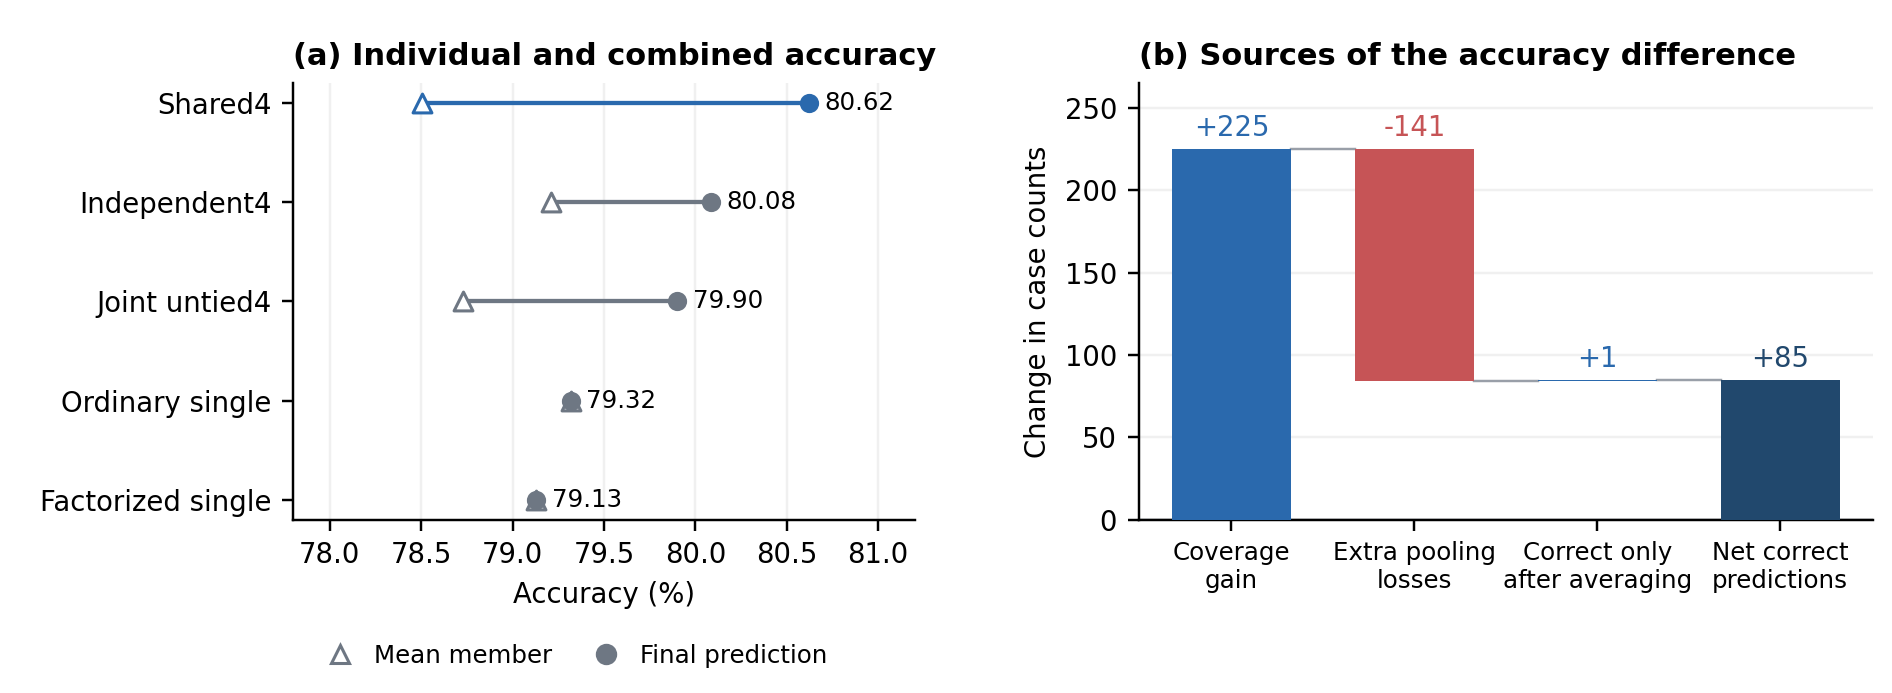
\includegraphics[width=\linewidth]{F_member_coverage_v2.png}
\caption{Internal SAGE on selected WikiCS development. (a) Shared4's average member is weaker than either complete ensemble control, while its combined prediction is more accurate. Both single-model references are shown. (b) Against independently acquired factorized models, 225 added covered cases are offset by 141 extra losses during averaging; one aggregation-only correction leaves 85 more correct decisions. Counts repeat the same 5,274 nodes across three optimizer seeds. The paired mean accuracy gain is 0.537 points, with a descriptive 95\% interval of $[-0.265,1.340]$; this is not unused confirmation or a statistically established superiority claim. Calibrated NLL is higher than that of the independent ensemble.}
\label{fig:internal-members-coverage}
\end{figure}

Shared4 has higher calibrated NLL than both ensemble controls, while calibrated Brier favors Shared4 over both. The accuracy benefit therefore accompanies a probability-quality tradeoff that differs across proper scores. Appendix~\ref{app:internal-sage-F} gives the absolute confidence metrics and the study's predeclared decision rules.

The main text reports the member/coverage comparison. Complete signed counts, gross repairs/harms and their original discussion remain in \path{code_evidence/native_F/complete_prediction_accounting.tex.txt}. These repeated-node diagnostics compare separately fitted and selected procedures and identify no general learning cause.

Fewer stored weights remain a secondary benefit: Shared4 has 216,674 parameters, versus 832,256 for the complete four-body controls. Its recorded acquisition sum is 71.676 seconds, versus 50.025 for joint untied4 and 58.620 for I4. These scopes include different stopping histories and do not establish lower latency. Full seed, confidence, error and cost records accompany the study.

\section{Conditional SAGE and packed development comparison}\label{app:E-PE}
The conditional comparison tests a change to the neighbor values while retaining native SAGE aggregation. All 15 banks and 24 optimizer/body acquisitions in E closed before the complete readout; all 75 temperature fits closed. A separate packed comparison adds three banks, three optimizer bundles and 12 private narrower bodies. The joined raw analysis therefore covers 18 banks, 27 acquisition bundles and 36 body records, without adding calibration, model forwards or selected-state deserializations.

\subsection{Operation, controls and acquisition}
All arms use the complete WikiCS graph (11,701 nodes, 300 features and ten classes), 580 TRAIN nodes and 5,274 development nodes, with seeds 7301, 7403 and 7507. BASE/E4/N4/equipped M1/I4 use two native residual SAGE blocks, width 128, LayerNorm and dropout 0.2. Internal BatchEnsemble factors wrap every native dense map; shared native biases remain outside the private output scales. Native first-input factors start with Rademacher signs, later factors at one, and each route has a persistent dropout stream.

For each factual nonself edge $u\to v$ and route $m$, E4's two $256\to16$ affine builders consume $z_{uv}^{(m)}=[h_u^{(m)},h_v^{(m)}]$. Their shared matrices and biases have private input/output factor vectors. Reshaping each output to $4\times4$ gives
\begin{equation}\label{eq:E-paired-maps}
F_{a,uv}^{(m)}=I_4+\tfrac12\tanh A_a^{(m)}(z_{uv}^{(m)}),\quad a\in\{\mathrm{src},\mathrm{tgt}\},\qquad
T_{v\leftarrow u}^{(m)}=F_{\mathrm{tgt},uv}^{(m)\top}F_{\mathrm{src},uv}^{(m)}.
\end{equation}
The product acts on the $4\times32$ source-value view before scalar mean aggregation. Self values, support and native root/neighbor affine maps, feed-forward order, normalization, dropout and classifier are retained. Builder weights/biases start at zero, so transport starts at identity; private builder factors start at one and acquire gradients after the builder weights move. This initialization supplies no learning guarantee. N4 uses $[h_v^{(m)},\operatorname{SiLU}(h_v^{(m)})]$ with the same builders and matrix action, built once per receiver rather than once per edge.

Shared banks minimize mean own cross-entropy; no pooled-loss gradient or auxiliary loss is added. AdamW uses learning rate 0.001 and zero decay, at most 1,000 updates and 300 stale updates. The selector keeps the earliest strict full-development accuracy maximum of the probability mean and restores model, optimizer and route streams. Equipped M1 has its own full loss and selector. Equipped I4 comprises four separately initialized, optimized, selected and restored M1 bodies with the same endpoint operation, followed by probability pooling. It has no reused M1 fit or learned-state cloning. These are complete acquisition procedures, with shared-bank and independent-body optimization/selection histories.

PE4 is a declared native SAGE adaptation of Packed-Ensembles with four untied width-59 bodies and $\gamma=1$. Dense maps, native biases, LayerNorms and heads are private, while parameter-free neighbor means are packed over member channels. Each body has complete hidden states and gradients. Mean own CE and one coherent pooled selector follow the same F training contract. Width is chosen by the full BASE parameter cap before scoring: width 59 gives 215,508 parameters; width 60 would give 221,560 and exceed the 216,674 cap. E4 has 21,966 more parameters than this packed reference. This fixed narrower context leaves the full-width equipped I4 quality comparison in place. The earlier F outcomes and original benchmark are retained separately; no historical cross-runtime F score supplies these fresh anchors.

\subsection{Complete selected outcomes}

\begin{table}[t]
\centering\small\setlength{\tabcolsep}{4pt}
\caption{Complete joined raw WikiCS development outcomes. Accuracy and member means are percentages, averaged over three optimizer seeds. NLL and Brier are lower-is-better. Every bank uses the native checkpoint-selection population.}
\label{tab:E-PE-raw}
\begin{tabular}{lrrrrr}
\toprule
Arm & Accuracy & Member mean & NLL & Brier & Parameters\\
\midrule
BASE (fresh shared4) & 80.6282 & 78.3766 & 1.137994 & 0.315096 & 216,674\\
E4 (endpoints) & 81.1971 & 79.4495 & 0.761107 & 0.297086 & 237,474\\
N4 (receiver) & 81.0517 & 79.5174 & 0.737769 & 0.295872 & 237,474\\
Equipped M1 & 80.2174 & 80.2174 & 0.765341 & 0.314952 & 225,600\\
Equipped I4 & 80.8937 & 80.2127 & 0.688787 & 0.293094 & 902,400\\
PE4 ($\gamma=1$, width 59) & 79.7876 & 78.4936 & 0.695566 & 0.306853 & 215,508\\
\bottomrule\end{tabular}\end{table}

Calibration divides the development nodes into five label-free folds of sizes 1,055/1,055/1,055/1,055/1,054, after native checkpoint selection used all 5,274 nodes. For each arm/seed/fold, one CPU float64 temperature fit completes 500 updates, with no retries or final whole-development refit. All 75 fits and 37,500 scalar updates closed. Out-of-fold calibration consequently does not create independent whole-pipeline evaluation. Calibration preserves member argmaxes but can change the probability mean. No PE temperature or calibrated PE endpoint was fitted.

\begin{table}[t]
\centering\small\setlength{\tabcolsep}{5pt}
\caption{Complete E-family calibrated development outcomes. Every entry is a three-seed mean. PE is absent because the joined comparison added no calibration.}
\label{tab:E-calibrated}
\begin{tabular}{lrrr}
\toprule
Arm & Calibrated accuracy (\%) & NLL & Brier\\
\midrule
BASE (fresh shared4) & 80.7294 & 0.685842 & 0.292675\\
E4 (endpoints) & 81.1971 & 0.652050 & 0.284499\\
N4 (receiver) & 81.0201 & 0.649441 & 0.284886\\
Equipped M1 & 80.2174 & 0.678221 & 0.297737\\
Equipped I4 & 80.9506 & 0.636007 & 0.283364\\
\bottomrule\end{tabular}\end{table}

\begin{table}[t]
\centering\small\setlength{\tabcolsep}{5pt}
\caption{E4 minus each E-family reference. Raw accuracy differences and descriptive paired-seed 95\% intervals are in percentage points; calibrated NLL differences are signed, with positive values worse. All raw seed differences are positive.}
\label{tab:E-paired}
\begin{tabular}{lrrr}
\toprule
Reference & Raw gain & Descriptive 95\% interval & Calibrated NLL change\\
\midrule
BASE & 0.5688 & $[0.1146,1.0231]$ & $-0.033791$\\
Equipped I4 & 0.3034 & $[-0.3560,0.9628]$ & $+0.016044$\\
N4 & 0.1454 & $[0.0015,0.2893]$ & $+0.002609$\\
Equipped M1 & 0.9796 & $[0.2124,1.7469]$ & $-0.026171$\\
\bottomrule\end{tabular}\end{table}

\paragraph{Predeclared screens and uncertainty.}
The E raw rule requires mean gains of at least 0.2 points against BASE and equipped I4, all three differences nonnegative and at least two positive. Endpoint attribution against N4 has the same sign rule and a mean margin of 0.1 points. Both accuracy screens pass. The separate calibrated-NLL guard allows mean harm at most 0.02 and each-seed harm at most 0.05 against BASE/I4; it also passes. Against I4, the three calibrated harms are 0.010782/0.024975/0.012375, with mean 0.016044 and descriptive interval $[-0.003271,0.035359]$. All three are harm despite passing the practical allowance. Raw and calibrated NLL and Brier favor I4. Calibrated accuracy favors E4 at two seeds, with mean gain 0.2465 points and descriptive interval $[-0.3712,0.8642]$.

These intervals use three paired optimizer repeats on one encountered graph ($t$, two degrees of freedom). They do not account for preceding design selection, multiple comparisons or variation across graphs. The raw exact two-sided sign-flip value is 0.25 for each E-family contrast. Node readouts and calibration folds are not independent graph trials. The I4 accuracy interval includes zero; a practical NLL allowance does not establish statistical noninferiority. Member quality and cost were diagnostics rather than post hoc vetoes. No test labels enter this development analysis, and no unused confirmation or novelty verdict follows.

\begin{table}[t]
\centering\small\setlength{\tabcolsep}{4pt}
\caption{All joined packed-context raw contrasts, candidate minus PE4. Gains and descriptive paired 95\% intervals are in percentage points. Positive NLL/Brier changes are worse. These contexts do not replace the E-family's predeclared full-width quality references.}
\label{tab:PE-contrasts}
\begin{tabular}{lrrrr}
\toprule
Candidate & Accuracy gain & Descriptive 95\% interval & NLL change & Brier change\\
\midrule
BASE (fresh shared4) & 0.8406 & $[0.7318,0.9494]$ & $+0.442429$ & $+0.008244$\\
E4 (endpoints) & 1.4094 & $[0.9820,1.8368]$ & $+0.065541$ & $-0.009767$\\
N4 (receiver) & 1.2641 & $[0.7560,1.7721]$ & $+0.042203$ & $-0.010981$\\
Equipped M1 & 0.4298 & $[-0.0228,0.8824]$ & $+0.069775$ & $+0.008099$\\
Equipped I4 & 1.1061 & $[0.8643,1.3478]$ & $-0.006779$ & $-0.013758$\\
\bottomrule\end{tabular}\end{table}


The BASE--PE and E4--PE raw screens pass the declared 0.2-point mean/sign rule. PE improves NLL over BASE/E4/N4/M1 but has worse NLL than I4; its Brier ordering also differs. One width/gamma choice supplies no uniform quality or whole-family ranking.

\subsection{Prediction accounting}
Covered alternatives are readouts with at least one correct member. A pooling loss is a covered alternative lost in the served probability mean. The counts below sum three dependent readouts of the same 5,274 nodes (15,822 readouts) and compare separately fitted/selected procedures; they are descriptive rather than causal events.

\begin{table}[t]
\centering\small\setlength{\tabcolsep}{4pt}
\caption{Complete net error accounting. Each row is candidate minus reference. Coverage and loss changes retain their signs; an aggregation-only correction has no individually correct member. Repairs/harms compare the two pooled decisions directly.}
\label{tab:E-PE-errors}
\begin{tabular}{lrrrrr}
\toprule
Contrast & Coverage & Pool losses & Pool-only & Net correct & Repairs/harms\\
\midrule
E4--BASE & $-106$ & $-196$ & 0 & 90 & 512/422\\
E4--N4 & $-12$ & $-35$ & 0 & 23 & 213/190\\
E4--equipped I4 & 44 & $-4$ & 0 & 48 & 475/427\\
E4--equipped M1 & 970 & 815 & 0 & 155 & 595/440\\
\midrule
BASE--PE4 & $+295$ & $+161$ & $-1$ & 133 & 773/640\\
E4--PE4 & $+189$ & $-35$ & $-1$ & 223 & 784/561\\
N4--PE4 & $+201$ & $+0$ & $-1$ & 200 & 729/529\\
Equipped M1--PE4 & $-781$ & $-850$ & $-1$ & 68 & 553/485\\
Equipped I4--PE4 & $+145$ & $-31$ & $-1$ & 175 & 531/356\\
\bottomrule\end{tabular}\end{table}

E4 improves members over BASE while coverage falls and fewer alternatives are lost in pooling; N4 serves 67 of E4's 90 additional BASE-correct readouts. The endpoint increment varies across classes. These are separately fitted/selected procedures, without private-builder or optimization attribution. Complete discussion is in \path{code_evidence/native_E_PE/complete_contrasts_and_accounting.tex.txt}.

\subsection{Recorded resource scopes}
\begin{table}[t]
\centering\small\setlength{\tabcolsep}{5pt}
\caption{Complete three-bank resource scopes. Acquisition and selected serving are sums in seconds; allocated peak is decimal GB. I4 peak is the maximum for a separately acquired complete member body. Timers include different stopping histories and overlap; they are not isolated latency benchmarks.}
\label{tab:E-PE-costs}
\begin{tabular}{lrrr}
\toprule
Arm & Acquisition sum & Selected serving sum & CUDA allocated peak (GB)\\
\midrule
BASE (fresh shared4) & 234.671 & 0.161034 & 1.162\\
E4 (endpoints) & 1566.748 & 1.325601 & 16.120\\
N4 (receiver) & 636.351 & 0.311309 & 4.018\\
Equipped M1 & 372.650 & 0.351277 & 4.652\\
Equipped I4 & 1487.302 & 1.293800 & 4.652\\
PE4 ($\gamma=1$, width 59) & 134.589 & 0.126955 & 1.020\\
\bottomrule\end{tabular}\end{table}

Sharing saves stored parameters against equipped I4, while E4's observed four-route activation peak is much larger than that of one separately acquired I4 body. The E acquisition overlapped other work on the same GPU, and the PE acquisition was a separate run. Stopping histories, selector calls, restores and serving scopes are retained; sums are not concurrent wall time, and lifetime RSS peaks are not per-arm allocations. Preparation and discarded qualification also incur cost. No lower compute, isolated latency or peak-memory claim follows from the parameter counts.

All original E calibration rules remain unchanged. PE adds raw endpoints only. The operation combines established mechanisms; the comparison does not isolate private builder factors from private route states or capacity.

\subsection{Error strata and anchored head diagnostic}\label{app:E-error-head}
A fixed diagnostic reads the archived E/BASE/N4/I4 decisions at seeds 7301/7403/7507 without changing them. The 15,822 readouts repeat 5,274 development nodes. A strict common rival is some false class strictly above truth in every member's raw scores, rather than a shared wrong argmax. Exact softmax preserves each strict ordering; any nonnegative scalar probability average preserves their common ordering. This limits unchanged member mixing, without proving absent hidden information or locating a representation/classifier bottleneck.

E4 has 2,064 strict-rival readouts, versus BASE's 1,929 and I4's 2,139. Of E4's 2,975 pooled errors, 815 lose a correct member alternative and 96 have neither a correct member nor a strict common rival. Against BASE, E4 removes 316 old rival predicates, serves 79 old-rival repairs and creates 451; against I4 it removes 436, serves 122 and creates 361. Predicate removal alone is not served repair. E4--I4's net +48 consists of +63/+45 for factual classes 2/8 and -60 elsewhere; five classes gain and five lose. E4--N4's +23 consists of +27 at incoming nonself degree 5--12 and -4 elsewhere. These post hoc marginals justify no class/degree router, monotone degree effect or causal source-context claim. Full cells, including empty/small strata, remain in \path{evidence/closed_E_strata_COUNTS.json}.

The completed head diagnostic holds the original eval-mode width-128 representations and original heads fixed for affine residual conditions. Across 18 restored E/M1/I4 bodies, 27 member trajectories retain all 580 TRAIN and 5,274 SELECT rows. E compares head-only BatchEnsemble continuation with common and private zero-initialized unrestricted affine residuals. M1/I4 receive equally processed continuation/affine controls; I4 retains four own optimizers/selectors. Every condition adds a learned score delta to the original stored-logit anchor, and original flags remain authority. Fresh AdamW moments, rate 0.001, zero decay, mean own CE, a 1,000-update cap and 300 stale updates reproduce the strict full-SELECT probability-mean selector. Steps 1--1,000 are eligible; untouched step 0 remains a separate reported anchor. There is no backbone update, calibration, feature scaling or class-specific fitting.

\begin{table}[t]
\centering\small\setlength{\tabcolsep}{4pt}
\caption{Complete anchored fixed-feature head diagnostic. Values are equal means across three optimizer seeds; accuracy/member means are percentages and raw pooled NLL is lower-is-better. Untouched references remain visible. All outcomes use the already selected development population.}
\label{tab:E-head-absolute}
\begin{tabular}{lrrrr}
\toprule
Condition & Accuracy & Member mean & Raw NLL & Strict rivals\\
\midrule
E4 untouched & 81.197067 & 79.449501 & 0.761106833 & 2064\\
E4 BE continuation & 81.178106 & 79.479522 & 0.777546617 & 2059\\
E4 common affine & 81.159145 & 79.449501 & 0.774839515 & 2061\\
E4 private affine & 81.190747 & 79.593288 & 0.780286927 & 2080\\
M1 untouched & 80.217419 & 80.217419 & 0.765340731 & 3130\\
M1 BE continuation & 80.299583 & 80.299583 & 0.772817430 & 3117\\
M1 affine & 80.312223 & 80.312223 & 0.771618117 & 3115\\
I4 untouched & 80.893692 & 80.212679 & 0.688786634 & 2139\\
I4 BE continuation & 80.912653 & 80.263241 & 0.694397369 & 2143\\
I4 private affine & 80.906333 & 80.271141 & 0.693524059 & 2142\\
\bottomrule\end{tabular}\end{table}

All 21 banks and 39 head optimizer bundles close. The frozen private-specific screen requires positive whole-SELECT private-minus-common and private-minus-BE accuracy at every seed, no worse mean member competence/NLL and positive mean improvement over untouched E. Correct-count vectors are $+3,-1,+3$ versus common, $+3,-3,+2$ versus BE and $+2,-3,0$ versus untouched E. Every accuracy clause fails. Mean member accuracy improves by 0.143787/0.113766 points versus common/BE, but pooled NLL worsens by 0.005447412/0.002740309 and by 0.019180094 versus untouched E. Per-member SELECT NLL was not exported for E/I4 and is unevaluable; pooled NLL does not substitute for it.

Private E has 50 own-anchor repairs and 51 harms. Coverage adds 45/removes 56 and pooling losses fall by 10, giving net -1 correct. On all 2,064 original E rival errors it obtains 40 correct-member alternatives and removes 46 predicates, yet loses all 40 in pooling and serves zero repairs. It creates 62 whole-population rival predicates, ending at 2,080. Common/BE also serve zero old-E-rival repairs. Private E remains above untouched M1/I4 by 0.973328/0.297055 points, but these advantages predate the head change; against affine-processed M1/I4 it gains 0.878524/0.284414 points, with I4 correct-count signs $+24,+27,-6$. Its NLL is worse than every original/processed reference. Private-minus-untouched-E class nets are $3,0,-21,8,-9,4,1,12,3,-2$, summing to -1; no favorable class rescues the failed screen.

The recorded complete scope is 74.54 seconds, process-lifetime peak RSS 943,833,088 bytes and CUDA allocation 1,569,668,608 bytes, with feature extraction/head fitting overlapping other work. These are not isolated speed or per-arm peaks. The earlier negative regularized Polynormer head-refit scope remains closed. This result closes the exact anchored affine recipe, without ruling out nonlinear information, stronger ordinary/end-to-end training or global capacity. Full protocol, absolute per-seed records, contrasts, factual classes, optimizer accounting and cost/replay receipts are in \path{evidence/closed_E_head_PLAN.json}, \path{evidence/closed_E_head_COMPLETE.json} and \path{evidence/closed_E_head_SUMMARY.json}. Numerical replay is an engineering record rather than a utility criterion; no unused whole-pipeline confirmation follows.

\section{Additional development objectives}\label{app:auxiliary-development}
The additional affinity and fixed-key studies did not establish a useful increment over their own unchanged shared baselines. Private affinity changes raw accuracy by $-0.006320$ points with mixed seed signs; private fixed keys change it by $-0.037922$ points with three negative signs and fail all five attribution checks. Their gains against equipped I4/single references remain visible, along with failed mean NLL protections. These distinct studies neither replace the F selected bank nor establish a successful auxiliary specialization mechanism.


\section{Complete heldout studies and native controls}\label{app:complete-confirmation-v5}
This section adds complete Physics/Penn and FiLM/association evidence after A14. Earlier numerical blocks remain unchanged. Full class grids, proper-score/member vectors, calibration endpoints, body costs and custody receipts are in \path{evidence/physics/}, \path{evidence/penn94/}, \path{evidence/film/} and \path{evidence/association/}. Values below transcribe released scalar records; no models or predictions were recomputed for this revision.

\subsection{Physics: acquisition, selection and scoring}\label{app:physics-v5}
The complete graph has 34,493 nodes, 8,415 raw binary float32 features and five classes. The pinned provider removes loops and coalesces undirected edges; exactly one self record per node is then added, giving 530,417 common support entries. Features are not row-normalized. Blocks are 8101/8219/8363/8501/8663/8819/9001/9199/9403/9623. For each class, a prospectively fixed NumPy RandomState permutation assigns 20 TRAIN, 30 SELECT, 30 CAL and the remainder TEST nodes; total roles are stated in Section~\ref{sec:physics}. These custom masks preserve the cited training/selection label budget while reserving additional calibration labels, without reproducing a canonical published split.

BASE/E4/N4 and equipped M1/I4 use two width-128 residual native SAGE blocks, LayerNorm, GELU, dropout 0.2 and AdamW at 0.001 with zero decay. E/N retain the WikiCS endpoint/receiver operators and factor law. Shared banks minimize mean own CE and choose the earliest strict maximum pooled SELECT accuracy; singles and each I4 body use their own full loss, optimizer and SELECT checkpoint. The cap is 1,000 updates with 300 stale updates. Four route states still require four graph passes. The source-derived mean-SAGE port instead uses width 32, depth two, dropout 0.4, Adam at 0.001, first-layer weight penalty 0.05, output row normalization and its native total-SELECT-loss selector with latest ties, 50 stale updates and a 100,000-update ceiling. It is a Torch source port with different acquisition opportunities, not a bitwise TensorFlow reproduction or matched-capacity control.

All ninety selected states and sixty prediction banks freeze before calibration. Each bank receives one positive temperature initialized at one and fitted for exactly 500 CPU float64 Adam updates on separate CAL (rate 0.01, zero decay, standard moments). The final update is the endpoint; there is no retry, grid or SELECT/CAL refit. Temperature acts on member log probabilities before averaging. All sixty endpoints freeze before one complete TEST-label release. Every native and readout outcome is finite, without replacement blocks or survivor means.

\begin{table}[t]
\centering\footnotesize\setlength{\tabcolsep}{3pt}
\caption{Complete Physics heldout outcomes. Accuracy is percent, mean $\pm$ sample SD across ten mask/optimizer blocks on one graph; proper scores are block means. Lower NLL/Brier is better.}
\label{tab:physics-absolute-v5}
\resizebox{\linewidth}{!}{%
\begin{tabular}{lrrrrrr}
\toprule
Procedure & Raw accuracy & NLL & Brier & Cal. accuracy & Cal. NLL & Cal. Brier\\
\midrule
BASE shared4 & $90.5403\pm0.6887$ & 0.330462 & 0.155794 & $90.5112\pm0.6877$ & 0.322773 & 0.152844\\
E4 & $91.3264\pm0.7243$ & 0.303481 & 0.140487 & $91.3258\pm0.7170$ & 0.291916 & 0.138634\\
N4 & $91.2982\pm0.7081$ & 0.300462 & 0.139682 & $91.2967\pm0.7039$ & 0.290985 & 0.138897\\
Equipped M1 & $92.2233\pm0.8247$ & 0.302642 & 0.129237 & $92.2233\pm0.8247$ & 0.261391 & 0.123701\\
Equipped I4 & $92.7891\pm0.5641$ & 0.235658 & 0.112491 & $92.7932\pm0.5596$ & 0.230580 & 0.112070\\
Source mean-SAGE M1 & $93.0590\pm0.5618$ & 0.945902 & 0.466481 & $93.0590\pm0.5618$ & 0.218625 & 0.106848\\
\bottomrule
\end{tabular}}
\end{table}
\begin{table}[t]
\centering\footnotesize\setlength{\tabcolsep}{3pt}
\caption{Physics member quality. Worst accuracy is averaged after taking the least accurate member within each block. Full member Brier, worst NLL and block vectors remain in ARM\_AGGREGATES.json and BANK\_ROWS\_*.json.}
\label{tab:physics-members-v5}
\resizebox{\linewidth}{!}{%
\begin{tabular}{lrrrr}
\toprule
Procedure & Mean accuracy & Worst accuracy & Raw mean NLL & Cal. mean NLL\\
\midrule
BASE shared4 & 85.1630 & 83.9389 & 0.582108 & 0.615819\\
E4 & 87.0671 & 86.0115 & 0.556157 & 0.533826\\
N4 & 87.0734 & 86.0027 & 0.575345 & 0.530059\\
Equipped M1 & 92.2233 & 92.2233 & 0.302642 & 0.261391\\
Equipped I4 & 92.2419 & 91.5349 & 0.301177 & 0.317548\\
Source mean-SAGE M1 & 93.0590 & 93.0590 & 0.945902 & 0.218625\\
\bottomrule
\end{tabular}}
\end{table}


\paragraph{Frozen inference and failure.}
The two raw integer-accuracy primary comparisons use one-sided paired $t$ tests of positive effect, Holm correction at 0.05, and separately require both observed gains to reach 0.2 points. The conjunction fails. Paired intervals have nine degrees of freedom; the conservative simultaneous pair uses 97.5\% two-sided intervals per contrast for family coverage at least 95\%. Inference conditions on split/optimizer randomness on one graph and assumes approximately independent normal block differences; nodes and graph domains are not its units. Observed practical margins do not prove population lower bounds above those margins.

\begin{table}[t]
\centering\footnotesize\setlength{\tabcolsep}{3pt}
\caption{Physics E4 minus each primary reference, in percentage points. Both are required; simultaneous intervals follow the frozen two-contrast Bonferroni rule.}
\label{tab:physics-inference-v5}
\resizebox{\linewidth}{!}{%
\begin{tabular}{lrllrl}
\toprule
Reference & Mean & Paired 95\% interval & Simultaneous interval & Holm $p$ & Result\\
\midrule
BASE shared4 & 0.786085 & $[0.554845,1.017325]$ & $[0.511621,1.060549]$ & 3.03081e-05 & PASS\\
Equipped I4 & -1.462764 & $[-1.874409,-1.051119]$ & $[-1.951355,-0.974172]$ & 0.999989 & FAIL\\
\bottomrule
\end{tabular}}
\end{table}
\begin{table}[t]
\centering\footnotesize\setlength{\tabcolsep}{3pt}
\caption{Full Physics raw paired correct-count vectors (E4 minus reference). Every difference uses 34,093 heldout nodes; multiplying by 100/34,093 gives its percentage-point difference. Counts are exact, with dependent nodes across masks.}
\label{tab:physics-vectors-v5}
\begin{tabular}{lrrr}
\toprule
Block & BASE & Equipped I4 & N4\\
\midrule
8101 & 232 & -329 & 81\\
8219 & 196 & -542 & 52\\
8363 & 209 & -375 & -16\\
8501 & 530 & -722 & 13\\
8663 & 270 & -630 & 1\\
8819 & 177 & -275 & -20\\
9001 & 181 & -724 & -68\\
9199 & 324 & -385 & 4\\
9403 & 356 & -258 & 117\\
9623 & 205 & -747 & -68\\
\bottomrule
\end{tabular}
\end{table}


The E--N conditional gate is closed. Its 0.028158-point mean, $[-0.097196,0.153513]$ paired interval, six positive/four negative differences and one-sided $p=0.311785$ also fail the 0.1-point observed margin and one-sided criterion. Calibrated accuracy is reported without a second primary test. All 1,024 sign assignments are a symmetry/exchangeability sensitivity, not randomized arm assignment or a replacement primary test. E--BASE one-/two-sided values are 0.0009765625/0.001953125; E--I4 values are 1/0.001953125; E--N values are 0.3232421875/0.646484375. Seed IDs guarantee neither distribution assumption. No all-positive-block veto was adopted.

The separate practical calibrated-NLL screen allows mean harm at most 0.02 and harm at most 0.05 in every block. E--BASE mean harm is $-0.030857$ and passes. E--I4 harms in block order are 0.041473/0.054739/0.114460/0.087009/0.061091/0.027264/0.064243/0.053981/0.047044/0.062059: mean 0.061336, with seven blocks above 0.05. Both protections fail; this screen is not statistical NLL noninferiority. Raw NLL and Brier also favor I4. E's mean members improve 1.904130 points over BASE but remain 5.174743 points weaker than I4. The source single's stronger accuracy accompanies poor raw NLL, which separate-CAL fitting substantially reduces.

\subsection{Penn94: internal factors and whole-recipe controls}\label{app:penn-v5}
Penn94 retains all 41,554 graph nodes, including 2,739 with missing targets, with 4,814 one-hot public features and 2,724,458 canonical support entries. The target column is excluded before public encoding. Official split-0 TRAIN and TEST memberships remain. Official VALID IDs are sorted and permuted with NumPy RandomState 11709; the first floor-half becomes CAL and the remainder SELECT, with sorted exports. Role sizes are in Section~\ref{sec:penn}. Ten optimizer blocks use base seeds 0/10000/20000/30000/40000/50000/60000/70000/80000/90000 on the same roles. Scorer-only CONFIRM truth is absent from model and calibration bundles.

The common width-128, two-block SAGE, dropout, optimizer, own-CE objective and strict SELECT-accuracy checkpoint rule follow Appendix~\ref{app:internal-sage-F-details}. Matched boundary sharing factorizes only input/output maps under common acquisition; internal sharing factorizes all native dense maps. Genuine I4 selects four complete internal-factor bodies independently. Original boundary GNNM retains native TABM one-logit BCE: Xavier bias-free boundary matrices, private biases, original global sequential random draws, four scaled member backwards and one AdamW update, improving divisible-by-ten checkpoint cadence, 300 stale updates and a 5,000-update cap. The declared raw-accuracy metric replaces the historical binary ROC-AUC convention for this task. Its contrast with internal CE/probability pooling compares whole recipes.

The source-derived LINKX point uses width 128, two layers, dropout 0.5, AdamW rate 0.01 and decay 0.001, 500 epochs, one initial adjacency and feature layer, native BatchNorm and log-softmax/NLL, and earliest strict SELECT-accuracy maximum. A paired seed is set once before construction and one native reset. This is one source-backed point, not optimized published-score reproduction; its achieved outcome supplies descriptive task context outside the tested families.

All one hundred native body attempts close before ninety bank/fusion scalar fits: seventy primary banks and twenty alternate pool endpoints on the same selected internal/matched boundary states. Positive temperature starts at one and completes exactly 500 CPU float64 Adam updates on separate CAL (rate 0.01, zero decay), using the final endpoint with no retry. This is separate-role calibration, not WikiCS five-fold cross-fitting. All endpoints freeze before one complete ninety-row CONFIRM release; native and calibration failures are zero. Alternate fusion adds no native fit or forward.

\begin{table}[t]
\centering\footnotesize\setlength{\tabcolsep}{3pt}
\caption{Complete Penn94 CONFIRM outcomes, including frozen same-state alternate fusions. Accuracy is percent, mean $\pm$ sample SD across ten optimizer blocks; proper scores are block means. Alternate pooling does not replace the primary procedure.}
\label{tab:penn-absolute-v5}
\resizebox{\linewidth}{!}{%
\begin{tabular}{lrrrrrr}
\toprule
Procedure & Raw accuracy & NLL & Brier & Cal. accuracy & Cal. NLL & Cal. Brier\\
\midrule
Internal shared4 (prob.) & $78.1535\pm0.2378$ & 1.013331 & 0.345355 & $78.2761\pm0.2447$ & 0.466889 & 0.302321\\
Original GNNM (logit) & $79.1334\pm0.5519$ & 1.674650 & 0.390026 & $79.1334\pm0.5519$ & 0.459772 & 0.296400\\
Matched boundary (prob.) & $77.8619\pm0.2906$ & 1.039658 & 0.352805 & $77.9691\pm0.2738$ & 0.472374 & 0.306436\\
Ordinary M1 & $74.5605\pm0.5051$ & 0.878342 & 0.405003 & $74.5605\pm0.5051$ & 0.524340 & 0.348345\\
Factorized M1 & $74.6121\pm0.3253$ & 1.071828 & 0.407535 & $74.6121\pm0.3253$ & 0.525665 & 0.349155\\
Genuine factorized I4 & $75.2993\pm0.4472$ & 0.560094 & 0.354856 & $75.4230\pm0.6389$ & 0.502748 & 0.332149\\
LINKX & $84.6852\pm0.2225$ & 0.624994 & 0.258140 & $84.6852\pm0.2225$ & 0.344407 & 0.217322\\
Internal shared4 (logit alt.) & $78.3019\pm0.2433$ & 1.374803 & 0.397004 & $78.3019\pm0.2433$ & 0.469358 & 0.304018\\
Matched boundary (logit alt.) & $77.9835\pm0.2740$ & 1.390613 & 0.403082 & $77.9835\pm0.2740$ & 0.474774 & 0.308111\\
\bottomrule
\end{tabular}}
\end{table}
\begin{table}[t]
\centering\footnotesize\setlength{\tabcolsep}{3pt}
\caption{Penn94 primary-bank member quality. Singles repeat their own predictor. All member Brier/NLL and worst-member quantities remain in PER\_BLOCK\_QUALITY.csv and COMPLETE\_CONFIRM\_V1.json.}
\label{tab:penn-members-v5}
\resizebox{\linewidth}{!}{%
\begin{tabular}{lrrrr}
\toprule
Procedure & Mean accuracy & Worst accuracy & Raw mean NLL & Cal. mean NLL\\
\midrule
Internal shared4 (prob.) & 76.7476 & 76.4956 & 1.795546 & 0.515779\\
Original GNNM (logit) & 77.6445 & 77.2128 & 2.134410 & 0.502339\\
Matched boundary (prob.) & 76.5768 & 76.3390 & 1.783515 & 0.517041\\
Ordinary M1 & 74.5605 & 74.5605 & 0.878342 & 0.524340\\
Factorized M1 & 74.6121 & 74.6121 & 1.071828 & 0.525665\\
Genuine factorized I4 & 74.5873 & 74.2720 & 0.869825 & 0.609871\\
LINKX & 84.6852 & 84.6852 & 0.624994 & 0.344407\\
\bottomrule
\end{tabular}}
\end{table}


\paragraph{Primary conjunction and closed secondary gate.}
All four raw contrasts require Holm-adjusted one-sided paired $t$ values at most 0.05 and observed gains at least 0.2 points. The three favorable contrasts do not rescue the original-GNNM loss. Four simultaneous intervals use 98.75\% two-sided intervals per contrast for conservative family coverage at least 95\%. Inference assumes approximately independent normal optimizer-block differences conditional on one graph; nodes and I4 bodies are not the units. The sign-sensitivity assumptions and restrictions above also apply. No all-ten-positive veto or stronger practical-margin null was adopted.

\begin{table}[t]
\centering\footnotesize\setlength{\tabcolsep}{3pt}
\caption{Penn94 internal shared4 probability mean minus each primary reference, in percentage points. All four contrasts are required.}
\label{tab:penn-inference-v5}
\resizebox{\linewidth}{!}{%
\begin{tabular}{lrllrl}
\toprule
Reference & Mean & Paired 95\% interval & Simultaneous interval & Holm $p$ & Result\\
\midrule
Original GNNM & -0.979907 & $[-1.490781,-0.469034]$ & $[-1.682464,-0.277351]$ & 0.99906 & FAIL\\
Factorized I4 & 2.854199 & $[2.546435,3.161963]$ & $[2.430960,3.277438]$ & 8.93074e-09 & PASS\\
Ordinary M1 & 3.592993 & $[3.170802,4.015184]$ & $[3.012393,4.173593]$ & 1.27059e-08 & PASS\\
Factorized M1 & 3.541473 & $[3.252422,3.830525]$ & $[3.143967,3.938980]$ & 1.00606e-09 & PASS\\
\bottomrule
\end{tabular}}
\end{table}
\begin{table}[t]
\centering\footnotesize\setlength{\tabcolsep}{3pt}
\caption{Full Penn94 primary raw correct-count vectors. Each row uses the same 9,705 CONFIRM nodes; multiplying by 100/9,705 gives its percentage-point difference. Internal shared4 probability mean is the candidate throughout.}
\label{tab:penn-vectors-v5}
\begin{tabular}{lrrrr}
\toprule
Base seed & Original GNNM & Factorized I4 & Ordinary M1 & Factorized M1\\
\midrule
0 & -87 & 270 & 383 & 379\\
10000 & -78 & 309 & 318 & 333\\
20000 & -30 & 231 & 437 & 390\\
30000 & -152 & 206 & 298 & 284\\
40000 & -123 & 328 & 360 & 334\\
50000 & -107 & 243 & 352 & 402\\
60000 & -247 & 255 & 270 & 293\\
70000 & -77 & 314 & 436 & 336\\
80000 & 0 & 302 & 339 & 361\\
90000 & -50 & 312 & 294 & 325\\
\bottomrule
\end{tabular}
\end{table}


All 1,024 sign assignments give one-/two-sided values 1/0.00390625 against original GNNM and 0.0009765625/0.001953125 against each other primary reference. The sensitivity's Holm values are 1 for original and 0.00390625 for each other reference; this does not reopen the primary decision. The secondary Holm family stays closed. No secondary practical margin was adopted. Its matched-placement and two same-state serving outcomes remain fully reported:

\begin{table}[t]
\centering\footnotesize\setlength{\tabcolsep}{3pt}
\caption{All frozen Penn94 secondary contrasts. Holm values remain visible but the failed primary conjunction closes their confirmatory family; no practical secondary margin was adopted.}
\label{tab:penn-secondary-v5}
\resizebox{\linewidth}{!}{%
\begin{tabular}{lr lrl}
\toprule
Contrast & Mean pp & Paired 95\% interval & Holm $p$ & Gate\\
\midrule
Internal prob.--matched prob. & 0.291602 & $[0.129103,0.454101]$ & 0.00426667 & CLOSED\\
Internal prob.--logit, same states & -0.148377 & $[-0.273766,-0.022988]$ & 1 & CLOSED\\
Boundary prob.--logit, same states & -0.121587 & $[-0.212979,-0.030194]$ & 1 & CLOSED\\
\bottomrule
\end{tabular}}
\end{table}
\begin{table}[t]
\centering\footnotesize\setlength{\tabcolsep}{3pt}
\caption{Full Penn94 secondary raw correct-count vectors. Columns follow Table~\ref{tab:penn-secondary-v5}; negative serving contrasts favor logit averaging on the same states.}
\label{tab:penn-secondary-vectors-v5}
\begin{tabular}{lrrr}
\toprule
Base seed & Matched placement & Internal pool & Boundary pool\\
\midrule
0 & 13 & -39 & 7\\
10000 & 57 & -33 & -25\\
20000 & 42 & 0 & 0\\
30000 & 13 & 2 & -28\\
40000 & 44 & -24 & -10\\
50000 & -15 & -11 & -8\\
60000 & 17 & -33 & -12\\
70000 & 45 & -14 & -29\\
80000 & 46 & 9 & 0\\
90000 & 21 & -1 & -13\\
\bottomrule
\end{tabular}
\end{table}


Secondary one-/two-sided sign sensitivities are 0.00390625/0.0078125, 0.98828125/0.03125 and 0.99609375/0.015625 in table order. Logit alternatives use probability-selected states; they do not validate a newly logit-selected pipeline or authorize a CONFIRM-selected rescue.

Internal shared4 minus I4 raw NLL is $+0.453237$ and raw Brier $-0.009501$; separate-CAL fitting changes the NLL difference to $-0.035860$. All four practical calibrated-NLL protections pass. Mean/max harms are $+0.007117/+0.020959$ against original GNNM, $-0.057451/-0.041965$ against ordinary M1, $-0.058776/-0.042595$ against factorized M1 and $-0.035860/-0.019757$ against I4; the full ten-block vectors are in \path{evidence/penn94/summary/SUMMARY.json}. This screen neither proves statistical noninferiority nor erases raw overconfidence. Original GNNM and LINKX remain stronger raw-accuracy references.

\subsection{Prediction acquisition and retention}\label{app:retention-v5}
\begin{table}[t]
\centering\footnotesize\setlength{\tabcolsep}{3pt}
\caption{Signed candidate-minus-reference accounting. Net correct equals coverage minus pooling-loss change plus aggregation-only change. Counts sum dependent readouts across ten Physics/Penn blocks or three WikiCS seeds. Both repairs and harms remain; these are separately acquired predictions.}
\label{tab:retention-v5}
\resizebox{\linewidth}{!}{%
\begin{tabular}{lrrrrl}
\toprule
Contrast & Coverage & Pool losses & Pool-only & Net & Repairs/harms\\
\midrule
Physics E--BASE & 626 & -2057 & -3 & 2680 & 5462/2782\\
Physics E--I4 & 4379 & 9369 & 3 & -4987 & 5620/10607\\
Penn internal--I4 & 5047 & 2277 & 0 & 2770 & 10723/7953\\
Penn internal--original GNNM & 152 & 1103 & 0 & -951 & 5140/6091\\
FiLM shared--I4 & 223 & -25 & 0 & 248 & 717/469\\
\bottomrule
\end{tabular}}
\end{table}

Physics E adds covered alternatives over I4 but loses many more during averaging; favorable coverage cannot rescue its served loss. Penn internal sharing improves mean members over I4 by 2.160227 points but loses 0.896960 points against original GNNM. Shared FiLM improves mean members by 0.436102 points. With Roman SAGE and WikiCS F, these outcomes prevent a universal weaker-member explanation. Accounting describes separately acquired predictions, without identifying a learning cause or proving that new routing can recover their gaps.

\subsection{Native FiLM on encountered development}\label{app:film-v5}
The native PyG 2.7 FiLM operator produces receiver-conditioned gamma/beta, applies messagewise ReLU before averaging, keeps factual self records and retains its native skip. Native maps receive the declared internal factors. It is richer than N4 and differs from E in operator, geometry and parameterization. The 11,701-node WikiCS graph, 580 TRAIN and 5,274 encountered development nodes, seeds 7301/7403/7507, width 128, depth two, dropout 0.2, AdamW at 0.001 with zero decay, own CE and probability averaging follow the fixed development recipe. Shared4 selects a coherent pooled checkpoint; M1 and four independent I4 bodies select their own checkpoints. The cap is 1,000 updates with 300 stale updates and earliest strict accuracy maxima.

All nine banks and eighteen fits close. Five-fold temperature calibration after native selection on all development nodes completes forty-five scalar fits of 500 updates each, all successful, without retry or final refit. This does not create unused whole-pipeline evaluation; no TEST is scored. Selected steps are 457/453/796 for M1 and 908/732/537 for shared4; I4 selects 552/420/352/524, 450/43/243/950 and 404/344/210/150 in seed order. Unequal stopping histories remain part of the procedures.

\begin{table}[t]
\centering\footnotesize\setlength{\tabcolsep}{3pt}
\caption{Complete native FiLM development means. Proper scores remain visible; capacity differs from E4 (237,474 parameters). Absolute per-seed/member outcomes are in PER\_SEED\_QUALITY.csv.}
\label{tab:film-absolute-v5}
\resizebox{\linewidth}{!}{%
\begin{tabular}{lrrrrrrr}
\toprule
Procedure & Raw acc. & NLL & Brier & Cal. acc. & Cal. NLL & Cal. Brier & Params\\
\midrule
FiLM M1 & 77.2153 & 2.009551 & 0.435415 & 77.2153 & 0.885407 & 0.362311 & 340,928\\
FiLM shared4 & 79.9836 & 1.345641 & 0.332611 & 79.9520 & 0.731659 & 0.307864 & 354,146\\
FiLM I4 & 78.4161 & 1.253124 & 0.353255 & 78.4035 & 0.774740 & 0.326544 & 1,363,712\\
\bottomrule
\end{tabular}}
\end{table}

\begin{table}[t]
\centering\footnotesize\setlength{\tabcolsep}{3pt}
\caption{E4 minus each FiLM procedure on the same development. Raw accuracy vectors/intervals are points, ordered 7301/7403/7507; intervals are descriptive paired $t$ intervals with two degrees of freedom. Lower NLL is better.}
\label{tab:film-contrasts-v5}
\resizebox{\linewidth}{!}{%
\begin{tabular}{llrlrr}
\toprule
Reference & Raw seed gains & Mean pp & Descriptive 95\% interval & Raw NLL & Cal. NLL\\
\midrule
FiLM M1 & 4.152446/3.659462/4.133485 & 3.981797 & $[3.287948,4.675647]$ & -1.248444 & -0.233356\\
FiLM shared4 & 0.948047/1.687524/1.004930 & 1.213500 & $[0.191276,2.235724]$ & -0.584535 & -0.079608\\
FiLM I4 & 2.483883/2.938946/2.919985 & 2.780938 & $[2.141442,3.420433]$ & -0.492018 & -0.122689\\
\bottomrule
\end{tabular}}
\end{table}


Raw/calibrated Brier changes for E--M1, E--shared4 and E--I4 are $-0.138330/-0.077812$, $-0.035525/-0.023364$ and $-0.056170/-0.042045$; all individual proper-score seed changes favor E in this fixed setup. E's mean-member advantages are 2.234231/1.855012/2.291114 points. Full calibrated accuracy, member and Brier vectors are in \path{evidence/film/summary/E_COMPARISONS.csv} and the twelve scalar/custody partitions. These are exploratory comparisons without multiplicity-adjusted superiority, capacity matching, published-score reproduction or unused confirmation. The tested weak FiLM single/independent cells do not settle its literature comparison.

Shared FiLM minus I4 raw gains are 1.535836/1.251422/1.915055 points, mean 1.567438, descriptive 95\% interval $[0.740361,2.394514]$. Mean-member gains are 0.331816/0.237012/0.739477, mean 0.436102. Shared mean/worst member accuracies are 77.594489/76.804450\%, versus I4's 77.158387/76.741246\%. Raw NLL changes are $-0.055634/+0.340428/-0.007243$, mean $+0.092517$; calibrated changes are $-0.054332/-0.020039/-0.054872$, mean $-0.043081$. Raw/calibrated Brier improve by 0.020645/0.018681. This is a bounded shared-ensemble benefit with a raw probability-quality tradeoff, not a state-of-the-art reference or new primitive.

\subsection{Source-context reassignment in selected WikiCS functions}\label{app:association-v5}
The diagnostic closes 36 served banks, 108 trajectories and eighteen selected-state restores, with zero GNN/head updates, calibration or TEST access. One common restricted nonzero cyclic mapping (seed 2026101101) reassigns source context over 10,721 eligible receiver groups and 430,563 nonself records. Actual neighbor VALUE states, receiver context, self records, support and local context/map multisets remain at each hook; 11,701 self records stay fixed. Layer-0 changes propagate downstream, so later preservation is relative to each variant's incoming states. This deliberate context/VALUE mismatch is not a validated conditional sampler, independent rematching or covariance removal, and supplies no assignment uncertainty or causal training attribution.

\begin{table}[t]
\centering\footnotesize\setlength{\tabcolsep}{3pt}
\caption{All source-context reassignment conditions. Accuracy changes are points and NLL changes are relative to each factual selected predictor. Repairs/harms sum three dependent readouts of the same 5,274 nodes.}
\label{tab:association-v5}
\resizebox{\linewidth}{!}{%
\begin{tabular}{llrrrrl}
\toprule
Arm & Layers & Accuracy & Change & NLL change & Member change & Repairs/harms\\
\midrule
E4 & layer0 & 81.140185 & -0.056883 & -0.000803123 & 0.017381 & 28/37\\
E4 & layer1 & 80.937935 & -0.259133 & 0.008384796 & -0.142207 & 77/118\\
E4 & both & 80.912653 & -0.284414 & 0.009121389 & -0.178549 & 99/144\\
equipped M1 & layer0 & 80.116294 & -0.101125 & 0.001526241 & -0.101125 & 44/60\\
equipped M1 & layer1 & 80.109973 & -0.107445 & 0.004115096 & -0.107445 & 33/50\\
equipped M1 & both & 80.008848 & -0.208570 & 0.006261950 & -0.208570 & 60/93\\
equipped I4 & layer0 & 80.887372 & -0.006320 & 0.002523635 & -0.118506 & 53/54\\
equipped I4 & layer1 & 80.843130 & -0.050563 & 0.001164010 & -0.067943 & 38/46\\
equipped I4 & both & 80.811528 & -0.082164 & 0.004377577 & -0.183289 & 71/84\\
\bottomrule
\end{tabular}}
\end{table}


Both-layer E/I4 mean-member losses are similar ($-0.178549/-0.183289$ points). Factual E--I4 served/coverage/pooling-loss gaps are 48/44/$-4$; after both-layer reassignment they become 16/59/43. E loses seventeen covered readouts and adds twenty-eight pooling losses; I4 loses thirty-two covered readouts and removes nineteen pooling losses. E layer 0 loses accuracy but improves NLL. Greater served E sensitivity therefore does not establish greater loss of available alternatives or ensemble-specific learning causality.

Both-layer E has 99 repairs/144 harms, removes 92 strict-rival predicates but creates 112, and ends with 2,084 versus 2,064 factual rival errors. On the original-rival cohort, 75 newly covered readouts yield five repairs because seventy alternatives are lost in pooling. Favorable cohorts/classes cannot rescue the full-population harm. Factual flags remain authority and full class/per-seed tables are bundled. No after-retraining necessity, private-builder attribution or recovered geometry follows.

\subsection{Complete costs and custody}\label{app:confirmation-costs-v5}
\begin{table}[t]
\centering\footnotesize\setlength{\tabcolsep}{3pt}
\caption{All distinct-body acquisition/selected-serving sums and maximum allocated CUDA peaks. Times are seconds, peaks decimal GB. Penn acquisition uses fit-wall sums; Physics/FiLM use native acquisition scopes; source-port serving includes archive export. I4 peaks describe separately acquired bodies. Timer scopes and overlap preclude speed rankings.}
\label{tab:confirmation-costs-v5}
\resizebox{\linewidth}{!}{%
\begin{tabular}{llrrrr}
\toprule
Study & Procedure & Bodies & Acquisition & Selected serving & Peak GB\\
\midrule
Physics & BASE shared4 & 10 & 1147.847 & 0.956556 & 3.707\\
Physics & E4 & 10 & 5869.184 & 5.038499 & 8.229\\
Physics & N4 & 10 & 2857.788 & 1.544626 & 4.647\\
Physics & Equipped M1 & 10 & 1395.572 & 1.274910 & 8.227\\
Physics & Equipped I4 & 40 & 5374.815 & 4.914061 & 8.195\\
Physics & Source mean-SAGE M1 & 10 & 463.736 & 0.672963 & 0.148\\
Penn94 & Internal shared4 (prob.) & 10 & 4461.374 & 1.355801 & 8.474\\
Penn94 & Original GNNM (logit) & 10 & 14144.841 & 1.353448 & 3.430\\
Penn94 & Matched boundary (prob.) & 10 & 4573.694 & 1.340847 & 7.127\\
Penn94 & Ordinary M1 & 10 & 391.654 & 0.307202 & 2.612\\
Penn94 & Factorized M1 & 10 & 515.699 & 0.346492 & 3.625\\
Penn94 & Genuine factorized I4 & 40 & 1908.580 & 1.387770 & 3.638\\
Penn94 & LINKX & 10 & 428.471 & 0.270565 & 1.304\\
WikiCS & FiLM M1 & 3 & 220.055 & 0.076084 & 2.169\\
WikiCS & FiLM shared4 & 3 & 776.144 & 0.278148 & 7.318\\
WikiCS & FiLM I4 & 12 & 697.369 & 0.327983 & 2.180\\
\bottomrule
\end{tabular}}
\end{table}


Physics's concurrent cohort owner takes 16,693.35 seconds. Custodial preprocessing is 64.501 seconds; core preparation is 11.275 seconds within the 16,691.662-second core acquisition/preparation scope; source-port acquisition is 472.702 seconds. These nested/concurrent scopes are not additive isolated wall times. Selected export, sixty calibration endpoints, CPU readout, saves/restores and earlier failed preparation/qualification receipts are in \path{evidence/physics/complete_closed_evidence/RESULT_METADATA.json} and \path{evidence/physics/complete_closed_evidence/PIPELINE_CLOSURE.json}. Earlier failed attempts remain distinct from the successful frozen native/readout roster. All ninety selected-state receipts are bound.

Penn \path{evidence/penn94/summary/ACQUISITION_COSTS.csv} retains all one hundred unique bodies, including training, selection, saves, restoration, serving, cached-pool and memory scopes. Twenty alternate fusions add no body fits. Complete native/calibration/scorer and owner receipts, actual configuration and runtime/source bindings are in \path{evidence/penn94/custody/}. FiLM retains eighteen fit/checkpoint records and nine bank archives, plus 22,500 scalar updates: fit-sum time 87.875 seconds nested in calibration wall 88.714 seconds. Source-association external/script times are 32.361/31.520 seconds, with lifetime RSS 849,264,640 bytes and CUDA allocation 1,942,688,768 bytes. Later work overlaps on one allocation GPU, preventing isolated efficiency rankings. Stored parameters, computation and allocation remain separate.

The scalar/custody bundle copies no datasets, native checkpoints or member-logit tensors; receipts bind original artifacts. \path{IMMUTABLE_DEPENDENCIES.json} pins every manuscript input and copied evidence source. Original numerical tables, figure bytes, nine relocated text tables and the V3 archive remain preserved. This complete evidence revision retains both failed conjunctions and does not activate a heldout-selected rescue or supply a novelty or manuscript-acceptance verdict.


\end{document}
